\documentclass[electronics,article,accept,moreauthors]{Definitions/mdpi}

%=================================================================
% MDPI internal commands
\firstpage{1}
\makeatletter
\setcounter{page}{\@firstpage}
\makeatother
\pubvolume{1}
\issuenum{1}
\articlenumber{0}
\pubyear{2026}
\copyrightyear{2026}
\datereceived{}
\daterevised{}
\dateaccepted{}
\datepublished{}
\setlength{\headheight}{20.0pt}

%=================================================================
% Title
\Title{Detecting GPS Spoofing Attacks with a Trust Index using Sensor Cross-Validation based on Inertial Information}
%\Title{Detection and Simulation of GPS Spoofing in Mobile Robots Using Sensor Cross-Validation}

% Authors
\Author{Nikhil Sarwara $^{1}$ and Ananda Maiti $^{2,}$*}

\AuthorNames{Nikhil Sarwara and Ananda Maiti}

\address{%
$^{1}$ \quad School of Information, Technology, Faculty of Science, Engineering and Built Environment, Deakin University, Burwood, VIC 3151, Australia; nikhilsarwara01@gmail.com\\
$^{2}$ \quad School of Information, Technology, Faculty of Science, Engineering and Built Environment, Deakin University, Waurn Ponds, VIC 3216, Australia;  anandamaiti@ieee.org
}

\corres{Correspondence: anandamaiti@ieee.org}

%=================================================================
% Abstract
\abstract{GPS spoofing poses a critical threat to autonomous mobile robots that rely on unencrypted civilian GPS signals for navigation. Although the PX4 autopilot's extended Kalman filter (EKF2) incorporates innovation gating to reject anomalous measurements, spoofed signals that emulate legitimate GPS characteristics with low reported error metrics can bypass this defence. This paper presents a sensor cross-validation framework that detects GPS spoofing by exploiting inconsistencies between GPS-reported velocity and IMU-derived angular dynamics. Eight heuristic labelling rules, including a novel GPS--IMU consistency discriminator, are defined to generate ground-truth annotations from MAVLink telemetry captured at 10 Hz. A Random Forest classifier trained on 30-sample sliding windows (15-sample stride) across 34 telemetry fields achieves 98\% classification accuracy with a 0.99 F1-score for normal-class identification on a dataset of 48,207 labelled records collected from PX4 SITL--Gazebo simulations under varied wind and spoofing conditions. The proposed GPS Trust Index provides a continuous real-time integrity metric complementary to the binary classifier output. The simulation results demonstrate that lightweight machine learning on existing autopilot telemetry can effectively augment EKF2-based discrimination, offering a deployable defence against civilian GPS spoofing without hardware modification.}

% Keywords
\keyword{GPS spoofing; unmanned aerial vehicles; sensor fusion; machine learning; anomaly detection; PX4 autopilot; IMU cross-validation; cyber-physical security}

%=================================================================
\begin{document}

%%%%%%%%%%%%%%%%%%%%%%%%%%%%%%%%%%%%%%%%%%
\section{Introduction}
\label{sec:introduction}

The proliferation of unmanned aerial vehicles (UAVs) and autonomous mobile robots across civilian, commercial, and industrial domains has created an urgent need for robust navigation security. Global Positioning System (GPS) receivers form the primary absolute positioning sensor for the vast majority of these platforms, providing global, continuous, and low-cost localisation at typical accuracies of 2--5 m for civilian code-phase receivers \citep{humphreys2012}. Civilian GPS signals on the L1 frequency (1575.42 MHz) are unencrypted, unauthenticated, and transmitted at extremely low power levels (approximately --130 dBm at the Earth's surface), making them susceptible to radio-frequency interference and, more critically, to structured spoofing attacks \citep{schmidt2016}.

Unlike jamming, which denies position information by overwhelming the receiver with noise, spoofing deceives the receiver into computing an incorrect position, velocity, and time solution by transmitting counterfeit GPS signals that the target receiver locks onto and tracks \citep{kerns2014}. The demonstrated consequences of successful spoofing attacks range from the subtle deviation of a ship's navigation log to the complete capture and control of an unmanned aerial vehicle \citep{humphreys2012}. Kerns et al. \citep{kerns2014} famously demonstrated that a civilian GPS spoofer could capture control of an unmanned aircraft mid-flight, forcing it to follow a trajectory determined by the attacker.

Modern autopilot systems such as the PX4 open-source autopilot employ sensor fusion through an extended Kalman filter (EKF2) that integrates measurements from GPS, inertial measurement units (IMUs), magnetometers, barometers, and other sensors \citep{px4docs}. The EKF2 applies innovation gating, a statistical test that rejects measurements whose residual exceeds a threshold derived from the estimated measurement covariance. This mechanism provides some defence against gross outliers but is fundamentally limited when the spoofed signal is carefully crafted: a sophisticated spoofer can generate signals whose innovation statistics fall within the expected bounds by emulating the measurement covariance that the EKF2 expects from a legitimate GPS solution.

The problem is compounded by the fact that the EKF2 weights GPS measurements based on the reported horizontal and vertical position error estimates ({\it eph} and {\it epv}). A spoofer that reports artificially low error metrics can gain disproportionate influence over the state estimate. The innovation gating threshold must balance sensitivity against false positives, and in practice, the window between a detectable and a deceptive spoof can be narrow enough that the filter accepts the compromised data before the gate closes.

This paper addresses three research questions:

\begin{enumerate}
\item \textbf{RQ1:} What specific vulnerabilities in the PX4 EKF2 sensor fusion architecture enable GPS spoofing attacks to remain undetected by existing onboard defences?
\item \textbf{RQ2:} Can a lightweight consistency discriminator between GPS-reported velocity and IMU-derived angular dynamics serve as a reliable spoofing indicator across varied flight conditions?
\item \textbf{RQ3:} To what extent can a GPS Trust Index provide a continuous, interpretable integrity metric that augments binary spoofing classification?
\end{enumerate}

To answer these questions, we developed a modular detection framework that operates exclusively on existing MAVLink telemetry streams captured at 10 Hz from a PX4 autopilot running in a software-in-the-loop (SITL) simulation with Gazebo. The framework applies a set of eight heuristic labelling rules, the most novel being a GPS--IMU consistency discriminator that exploits the physical principle that wind turbulence affects both sensors symmetrically while spoofing introduces velocity discrepancies that are inconsistent with the vehicle's angular dynamics. These heuristic labels serve as ground truth for training a Random Forest classifier on 30-sample sliding windows across 34 telemetry fields.

The paper is structured as follows. Section~\ref{sec:litreview} reviews the relevant literature on GPS fundamentals, spoofing attack vectors, existing detection approaches, and the PX4 EKF2 architecture. Section~\ref{sec:systemdesign} describes the system architecture and the GPS--IMU consistency discriminator in detail. Section~\ref{sec:methodology} presents the simulation environment, data capture pipeline, preprocessing steps, heuristic labelling scheme, and machine learning methodology. Section~\ref{sec:results} presents experimental results and analysis. Section~\ref{sec:discussion} discusses implications and limitations. Section~\ref{sec:conclusions} concludes the paper and outlines directions for future work.

%%%%%%%%%%%%%%%%%%%%%%%%%%%%%%%%%%%%%%%%%%
\section{Literature Review}
\label{sec:litreview}

\subsection{GPS Fundamentals and Vulnerabilities}
\label{sec:gpsfundamentals}

The Global Positioning System is a space-based radio-navigation system operated by the United States Space Force that provides positioning, navigation, and timing (PNT) services to civilian and military users worldwide. The civilian GPS signal, known as the Coarse/Acquisition (C/A) code, is transmitted on the L1 frequency at 1575.42 MHz using direct-sequence spread spectrum (DSSS) modulation with a 1.023 MHz chip rate \citep{yuan2023}. The signal structure is publicly documented in the IS-GPS-200 standard, which specifies the navigation message format, spreading codes, and signal characteristics in detail.

Several inherent characteristics of civilian GPS make it vulnerable to attack. The signal power at the Earth's surface is approximately --130 dBm, well below the thermal noise floor of --111 dBm for a typical 2 MHz bandwidth \citep{humphreys2012}. Civilian receivers have no mechanism to authenticate the origin of a GPS signal: the C/A code spreading sequences are publicly known and can be generated by any commercial-off-the-shelf software-defined radio. The navigation message contains no cryptographic authentication in its civilian format, meaning that any transmitter capable of generating a GPS-like signal structure can produce a signal that a civilian receiver will acquire, track, and treat as legitimate.

The security architecture of GPS distinguishes between the civilian C/A-code service and the military P(Y)-code and M-code services, which use encrypted spreading codes and cryptographic authentication. These military services are unavailable on civilian receivers, and backwards compatibility requirements prevent their adoption on the L1 C/A frequency. The modernised L2C and L5 civilian signals offer improved performance but similarly lack authentication in their baseline configurations. GPS III satellites transmit the L1C signal, which incorporates the Chimera authentication mechanism \citep{schmidt2016}, but widespread receiver support remains years away.

\subsection{Spoofing Attack Vectors}
\label{sec:spoofingvectors}

GPS spoofing attacks can be classified along several dimensions, including attacker capability, attack strategy, and target platform. Humphreys et al. \citep{humphreys2012} provided the first detailed public demonstration of a portable civilian GPS spoofer constructed from a software-defined radio, a power amplifier, and a control antenna. Their spoofer generated counterfeit GPS signals that a consumer-grade receiver locked onto and tracked, causing the receiver to report a false position while the attacker maintained signal lock through a gradual power and code-phase alignment strategy.

Kerns et al. \citep{kerns2014} extended this work to the domain of unmanned aircraft, demonstrating that a mid-flight UAV could be captured through GPS spoofing alone. Their attack began with the spoofer transmitting signals synchronised with the legitimate GPS constellation, then gradually increasing power until the target receiver's tracking loops locked onto the counterfeit signal. Once lock was achieved, the attacker could manipulate the navigation solution to steer the aircraft along an arbitrary trajectory. The attack was executed against a commercial UAV autopilot without any hardware modification, highlighting the practical severity of the threat.

The principal attack variants identified in the literature include:

\begin{enumerate}
    \item \textbf{Simple spoofing} transmits counterfeit GPS signals without synchronisation to the legitimate constellation, relying on the target receiver being in acquisition mode or on the spurious signal being sufficiently powerful to capture the tracking loops. This approach is detectable through signal monitoring but requires minimal attacker capability.
    
    \item \textbf{Carry-off spoofing} begins with the attacker synchronising their signal to the legitimate constellation at the target location, then gradually increasing transmission power and introducing small deviations in the navigation solution. The gradual drift allows the receiver's tracking loops and navigation filter to adjust incrementally, avoiding the large innovations that would trigger anomaly detection \citep{kerns2014}.
    
    \item \textbf{Meaconing} involves the reception, delay, and retransmission of legitimate GPS signals. The delayed retransmission causes the target receiver to compute an offset position. Meaconing attacks are simpler to execute than coherent spoofing but are also more readily detected through signal timing analysis.
    
    \item \textbf{Multi-vehicle spoofing} targets multiple receivers simultaneously using a single spoofer, which is particularly relevant for swarms of UAVs or fleets of autonomous vehicles. The spoofer transmits a single counterfeit signal that all nearby receivers track, causing them all to compute the same false position.
\end{enumerate}

\subsection{Existing Detection Approaches}
\label{sec:detectionapproaches}

Research on GPS spoofing detection spans cryptographic, physical-layer, software-based, and sensor-fusion approaches, each with distinct trade-offs between detection capability, deployment cost, and operational impact.

\begin{itemize}
    \item \textbf{Cryptographic approaches} address the root cause of GPS spoofing by adding authentication to the GPS signal structure. The U.S. government's M-code provides cryptographic authentication but is restricted to military receivers. The European Galileo system's Open Service Navigation Message Authentication (OSNMA) provides a publicly available authentication mechanism by appending digital signatures to the navigation message, and the GPS III Chimera mechanism similarly adds authentication to the L1C signal \citep{schmidt2016}. These approaches are effective in principle but require receiver hardware upgrades and are not available for the L1 C/A signals that dominate the civilian receiver market.
    
    \item \textbf{Physical-layer approaches} detect spoofing by analysing signal characteristics that are difficult for an attacker to emulate precisely. Angle-of-arrival (AOA) monitoring uses an antenna array to detect inconsistencies in the direction of signal arrival \citep{magiera2015}. Automatic gain control (AGC) monitoring detects the abnormal power levels characteristic of spoofing attacks. Correlator output analysis examines the shape of the correlation function between the received signal and the local replica: a spoofed signal produces distinct correlator distortions compared with authentic signals. These methods are effective but require hardware modifications, additional antennas, or specialised RF front-ends that are impractical for small UAVs.
    
    \item \textbf{Software-based approaches} operate on the navigation solution or raw measurements produced by the GPS receiver without requiring hardware changes. Receiver autonomous integrity monitoring (RAIM) detects faults by checking consistency among redundant satellite measurements, but RAIM cannot detect attacks that affect multiple satellites simultaneously, as most spoofing attacks do. Signal quality monitoring (SQM) analyses the shape of the correlation peak to detect distortion, but this requires access to correlator outputs that consumer-grade receivers do not expose.

\item \textbf{Sensor-fusion approaches} exploit the discrepancy between GPS measurements and other on-board sensors to detect spoofing. Magiera and Katulski \citep{magiera2015} surveyed spatial processing techniques that use antenna arrays to detect interference, while Tanil et al. \citep{tanil2018} proposed using IMU--GPS cross-correlation for spoofing detection in ground vehicles. Manesh et al. \citep{manesh2019} demonstrated that a neural network trained on GPS and IMU features could detect spoofing attacks in UAVs with high accuracy. The sensor-fusion approach is attractive because it leverages sensors already present on virtually all autonomous platforms and requires no hardware modifications.
  
\end{itemize}

\subsection{PX4 Architecture and EKF2}
\label{sec:px4architecture}

The PX4 autopilot is an open-source flight control software stack that runs on a wide range of hardware platforms, from small racing drones to full-scale unmanned aircraft. The software architecture is modular, with separate processes for sensor drivers, the attitude and position estimator, the flight controller, and the navigator, all communicating via a publish--subscribe message bus \citep{px4docs}.

The EKF2 estimator is a 24-state extended Kalman filter that fuses measurements from up to nine sensor types, including GPS position and velocity, IMU angular rates and accelerations, magnetometer heading, barometric pressure, optical flow, and external vision pose estimates. The filter runs at the IMU rate (typically 250--1000 Hz) for prediction steps and processes measurement updates at the individual sensor rates. The state vector includes, among others, the three-dimensional position, velocity, and attitude; gyroscope and accelerometer biases; wind estimates; and magnetic field components \citep{px4docs}.

The EKF2's defence against anomalous measurements is the innovation gating mechanism. For each measurement update, the filter computes the innovation (the difference between the predicted measurement and the actual measurement) and its covariance. If the squared Mahalanobis distance of the innovation exceeds a threshold derived from the chi-squared distribution, the measurement is rejected. The default innovation gate size for GPS position and velocity measurements is configured through the EKF2\_GATE\_POS and EKF2\_GATE\_VEL parameters, with typical values corresponding to a 99\% confidence interval \citep{px4docs}.

The critical vulnerability exploited by spoofing attacks is the GPS weighting mechanism. Each GPS measurement carries reported horizontal and vertical position error estimates ({\it eph} and {\it epv}), which the EKF2 uses to compute the measurement covariance matrix for the Kalman gain calculation. A spoofed signal that reports optimistically low {\it eph} and {\it epv} values receives disproportionately high weight in the state estimate. Furthermore, a carefully executed carry-off attack can introduce position drift that stays within the innovation gate by several metres per epoch, accumulating a significant position offset before the filter detects the anomaly.

The innovation gating is also limited by its reliance on the estimated measurement covariance, which depends on the filter's own state uncertainty. Once the filter has converged on the true state with low uncertainty, the innovation gate is tight. However, during high-dynamic manoeuvres or in the presence of turbulence, the state uncertainty increases, widening the gate and creating a window of opportunity for a spoofing attack to inject false measurements.

\subsection{Research Gaps}
\label{sec:researchgaps}

Based on the analysis of existing detection approaches and the PX4 EKF2 architecture, the following research gaps are identified:

\begin{enumerate}
\item \textbf{Cross-modal inconsistency exploitation.} While sensor-fusion approaches have been explored for spoofing detection, the specific physical relationship between GPS-reported velocity and IMU-derived angular dynamics -- namely, that wind turbulence affects both sensors symmetrically while spoofing affects only the GPS -- has not been systematically exploited for heuristic labelling or as a standalone discriminator.

\item \textbf{Limited evaluation of heuristic labelling for ML training.} Existing machine learning approaches to spoofing detection either use synthetically generated labels from simplistic assumptions or require manual labelling, which is impractical for the large datasets needed to train robust classifiers. The use of a diverse set of heuristics to generate reliable ground-truth labels without manual intervention has not been thoroughly investigated.

\item \textbf{Real-time deployability on existing PX4 hardware.} Many proposed detection algorithms require computational resources or sensor modalities that exceed what is available on typical PX4-based flight controllers. The feasibility of deploying a lightweight classifier on the existing 10 Hz MAVLink telemetry stream without modifications to the autopilot firmware remains an open question.

\item \textbf{Absence of a continuous trust metric.} Existing detection approaches produce binary classifications (spoofed or legitimate) without providing a continuous measure of GPS integrity that could inform higher-level decision-making, such as graceful degradation, mode switching, or operator alerting.

\item \textbf{Simulation-to-reality transfer validation.} Most evaluations of spoofing detection in UAVs are conducted either purely in simulation or exclusively in field trials with expensive hardware. Methodologies that bridge the gap between high-fidelity simulation and real-world deployment, ensuring that detectors trained in simulation transfer effectively, are insufficiently developed.
\end{enumerate}

%%%%%%%%%%%%%%%%%%%%%%%%%%%%%%%%%%%%%%%%%%
\section{System Design and Architecture}
\label{sec:systemdesign}

\subsection{Overall Architecture}
\label{sec:architecture}

The proposed detection framework follows a modular pipeline architecture comprising eight subsystems, each implemented as an independent Python module communicating through structured data interfaces. The high-level architecture proceeds as follows: PX4 SITL generates flight telemetry transmitted via MAVLink over UDP; the GPS Monitor captures eight message types at 10~Hz and writes structured CSV logs; the ML Pipeline processes raw CSVs through cleaning, feature engineering, heuristic labelling, sliding window creation, and model training; the Live Inference Engine consumes streaming telemetry and outputs anomaly probabilities; and the Streamlit Dashboard displays live metrics.

\begin{enumerate}
\item \textbf{GPS Monitor} ingests raw MAVLink GPS\_RAW\_INT messages and computes derived quantities, including Haversine distance between successive position reports, velocity magnitude, horizontal and vertical dilution of precision, satellite count, and error estimates ({\it eph}, {\it epv}).
\item \textbf{IMU Monitor} processes SCALED\_IMU and SCALED\_IMU2 messages to extract angular rates, linear accelerations, vibration metrics, and temperature readings. The module applies low-pass filtering to remove high-frequency noise while preserving dynamic manoeuvre signatures.
\item \textbf{Estimator Monitor} captures ESTIMATOR\_STATUS messages that contain the EKF2's internal innovation values, state covariance estimates, and status flags. This module provides direct insight into the filter's confidence in its own state estimate for each measurement type.
\item \textbf{Data Capture Pipeline} records all incoming MAVLink messages at 10 Hz into a synchronised time-series database. Each record carries a hardware-timestamped MAVLink system time and is indexed by flight session, simulation scenario, and message sequence number.
\item \textbf{Heuristic Labelling Engine} applies the eight heuristic rules (Section~\ref{sec:heuristics}) to each row of the captured dataset, producing a binary ground-truth label and a GPS Trust Index value.
\item \textbf{Machine Learning Pipeline} performs feature engineering, sliding-window segmentation, train--test splitting with flight-level isolation, model training, and hyperparameter optimisation.
\item \textbf{Live Inference Module} loads a trained classifier and GPS Trust Index calculator, processes incoming MAVLink telemetry in real time, and publishes classification results and trust index values to the MAVLink message bus as raw status messages.
\item \textbf{Streamlit Dashboard} provides a real-time visualisation interface displaying the classifier output, GPS Trust Index time series, heuristic rule activations, and telemetry data. A curses-based TUI (text user interface) companion provides a lightweight terminal-based alternative for headless deployment.
\end{enumerate}

\begin{figure}[H]
    \centering
    \includegraphics[width=0.85\textwidth]{figures/architecture image with calibiri font.png}
    \caption{Data flow from the PX4 simulation through the GPS Monitor, machine learning pipeline, and live inference system.}
    \label{fig:architecture}
\end{figure}  
  
  The modular design (as shown in Figure ~\ref{fig:architecture}) allows each subsystem to be developed, tested, and deployed independently. The heuristics engine and ML pipeline can be run offline for training, while the live inference module is a lightweight Python script that can run on the companion computer of a PX4-based UAV or as a ground-station process. The attack injection interface is shown in Figure~\ref{fig:attack_dashboard}.
  
\begin{figure}[H]
    \centering
    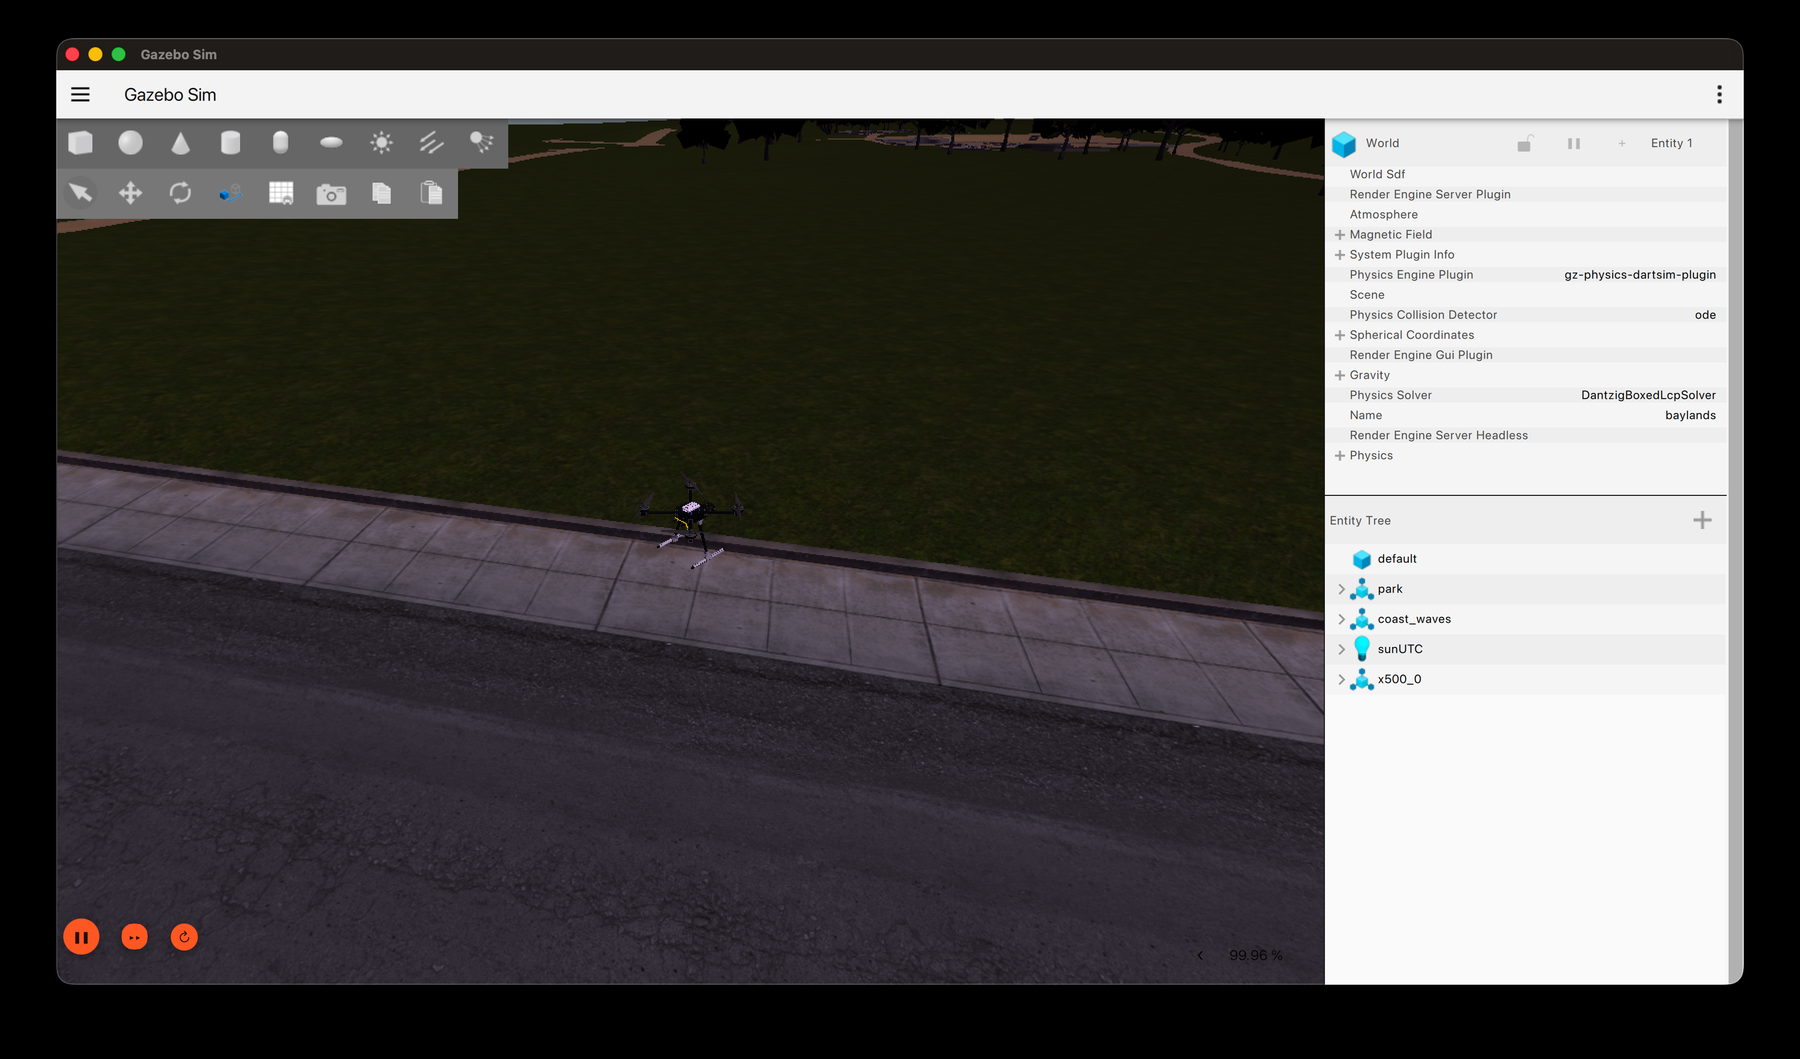
\includegraphics[width=0.95\textwidth]{figures/px4_simulation_gazebo.png}
    \caption{Attack injector and dashboard used to generate controlled GPS spoofing attacks for testing and evaluation.}
    \label{fig:attack_dashboard}
\end{figure}


\subsection{GPS--IMU Consistency Discriminator}
\label{sec:discriminator}

The core technical contribution of this work is the GPS--IMU consistency discriminator, a heuristic that exploits the differential effect of wind turbulence versus GPS spoofing on the relationship between GPS-reported velocity and IMU-measured angular dynamics.

The physical insight underlying the discriminator is as follows. When a UAV experiences wind gusts or atmospheric turbulence, the disturbance affects the airframe mechanically: the wind exerts forces and moments that cause both linear acceleration and angular rotation of the vehicle. The GPS receiver measures the resultant linear velocity through changes in the carrier phase and code phase of the received satellite signals, while the IMU gyroscopes measure the angular velocity directly. Thus, under authentic conditions, there exists a physical correlation between the UAV's linear velocity magnitude and its angular rate magnitude, mediated by the aerodynamic response of the airframe to atmospheric disturbances.

In a spoofing attack, the attacker injects counterfeit GPS signals that cause the receiver to report a false velocity. This false velocity is generated by the spoofer's arbitrary waveform generator and bears no relationship to the actual physical dynamics of the vehicle. The IMU, measuring true angular rates, is unaffected by the spoofing attack. Therefore, the correlation between GPS-reported velocity and IMU-measured angular rate is disrupted: the GPS reports high velocity (as dictated by the spoofing attack) while the IMU reports low angular rates (reflecting the actual steady flight condition).

The discriminator computes the following angular displacement metric from the three-axis gyroscope readings:

\begin{equation}
\|\boldsymbol{\omega}_{\text{all}}(t)\| = \sqrt{\omega_x(t)^2 + \omega_y(t)^2 + \omega_z(t)^2}
\label{eq:angularrate}
\end{equation}

where $\omega_x$, $\omega_y$, and $\omega_z$ are the angular velocities about the body-frame x (roll), y (pitch), and z (yaw) axes, respectively, measured by the IMU gyroscopes at time $t$. The magnitude $\|\boldsymbol{\omega}_{\text{all}}\|$ captures the total angular motion of the vehicle, including both deliberate manoeuvres and turbulence-induced rotations.

The GPS--IMU consistency condition is evaluated at each time step:

\begin{equation}
S(t) = \begin{cases}
1 & \text{if } \|\boldsymbol{\omega}_{\text{all}}(t)\| < \tau_\omega \text{ and } \|\mathbf{v}_{\text{GPS}}(t)\| > \tau_v, \\
0 & \text{otherwise},
\end{cases}
\label{eq:spoofindicator}
\end{equation}

where $\|\mathbf{v}_{\text{GPS}}(t)\|$ is the GPS-reported ground speed magnitude at time $t$, $\tau_\omega = 0.05$~rad/s is the angular rate threshold, and $\tau_v = 5.0$~m/s is the velocity threshold. When $S(t) = 1$, the discriminator flags the GPS reading as potentially spoofed, providing a heuristic ground-truth label for supervised learning.

The magnitude difference between GPS and IMU-derived motion can be expressed as:

\begin{equation}
\Delta\Phi(t) = \left| \|\mathbf{v}_{\text{GPS}}(t)\| - \alpha \cdot \|\boldsymbol{\omega}_{\text{all}}(t)\| \right|
\label{eq:deltaphi}
\end{equation}

where $\alpha$ is a scaling factor that maps angular rate to an equivalent linear velocity based on the vehicle's geometry. While $\Delta\Phi$ is useful as a continuous anomaly metric, the binary indicator in Equation~\ref{eq:spoofindicator} provides a cleaner training label by eliminating the dependence on the platform-specific scaling factor $\alpha$.

\textbf{Numerical example:} Consider two scenarios that illustrate the discriminator's operation.

\textit{Scenario A -- Spoofing without wind:} The UAV is in steady level flight with negligible angular motion. The IMU reports $\|\boldsymbol{\omega}_{\text{all}}(t)\| = 0.02$~rad/s, which is below $\tau_\omega$. The spoofed GPS reports $\|\mathbf{v}_{\text{GPS}}(t)\| = 10$~m/s, well above $\tau_v$. The condition $S(t) = 1$ is triggered, correctly labelling this as spoofing. The magnitude difference is $\Delta\Phi(t) \approx 10$~m (assuming $\alpha \cdot \|\boldsymbol{\omega}_{\text{all}}\| \ll \|\mathbf{v}_{\text{GPS}}\|$), providing a strong anomaly signal.

\textit{Scenario B -- Wind gust without spoofing:} The UAV encounters a wind gust that induces both linear and angular motion. The GPS reports $\|\mathbf{v}_{\text{GPS}}(t)\| = 6$~m/s, and the IMU reports $\|\boldsymbol{\omega}_{\text{all}}(t)\| = 0.15$~rad/s. Although the velocity exceeds $\tau_v$, the angular rate also exceeds $\tau_\omega$, so $S(t) = 0$: the discriminator correctly recognises that both sensors are responding consistently to a physical disturbance. The magnitude difference is $\Delta\Phi(t) \approx 0.2$~m, reflecting the correlated response.

The thresholds $\tau_\omega = 0.05$~rad/s and $\tau_v = 5.0$~m/s were selected empirically based on analysis of the training dataset. The angular rate threshold of 0.05~rad/s corresponds approximately to the noise floor of the IMU gyroscopes during steady flight, distinguishing between genuine angular motion (above threshold) and sensor noise (below threshold). The velocity threshold of 5.0~m/s was chosen to be above the typical ground speed during hover and low-speed manoeuvres while remaining sensitive to spoofed velocities that would typically be injected at higher values to achieve effective trajectory control.

A GPS Trust Index (GTI) is derived from the discriminator as a continuous measure of GPS integrity:

\begin{equation}
\text{GTI}(t) = 1 - \frac{1}{1 + \exp\left(-k \cdot (\|\mathbf{v}_{\text{GPS}}(t)\| - \tau_v)\right)} \cdot \frac{1}{1 + \exp\left(k \cdot (\|\boldsymbol{\omega}_{\text{all}}(t)\| - \tau_\omega)\right)}
\label{eq:gti}
\end{equation}

where $k$ is a steepness parameter controlling the transition sharpness. The GTI ranges from 0 (low trust, likely spoofed) to 1 (high trust, likely authentic). The two sigmoid factors capture the velocity and angular rate conditions respectively: the GTI approaches 0 when velocity is high and angular rate is low (the spoofing signature), and approaches 1 when either velocity is low (no spoofing possible) or angular rate is high (consistent with manoeuvring or turbulence).

The physical interdependence established by the discriminator is directly reflected in the downstream machine learning model's architectural focus. As visualized in Figure~\ref{fig:feature_importance}, an empirical feature evaluation reveals that GPS velocity magnitude (\texttt{vel\_m\_s}) along with IMU roll and pitch angular rates dominate the classifier's split selections. This structural prioritization validates the design of the physical consistency condition; when a spoofing attack disrupts the cross-modal correlation between these specific sensors, it creates an out-of-distribution signature that the ensemble trees can immediately isolate.

\begin{figure}[htbp]
\centering
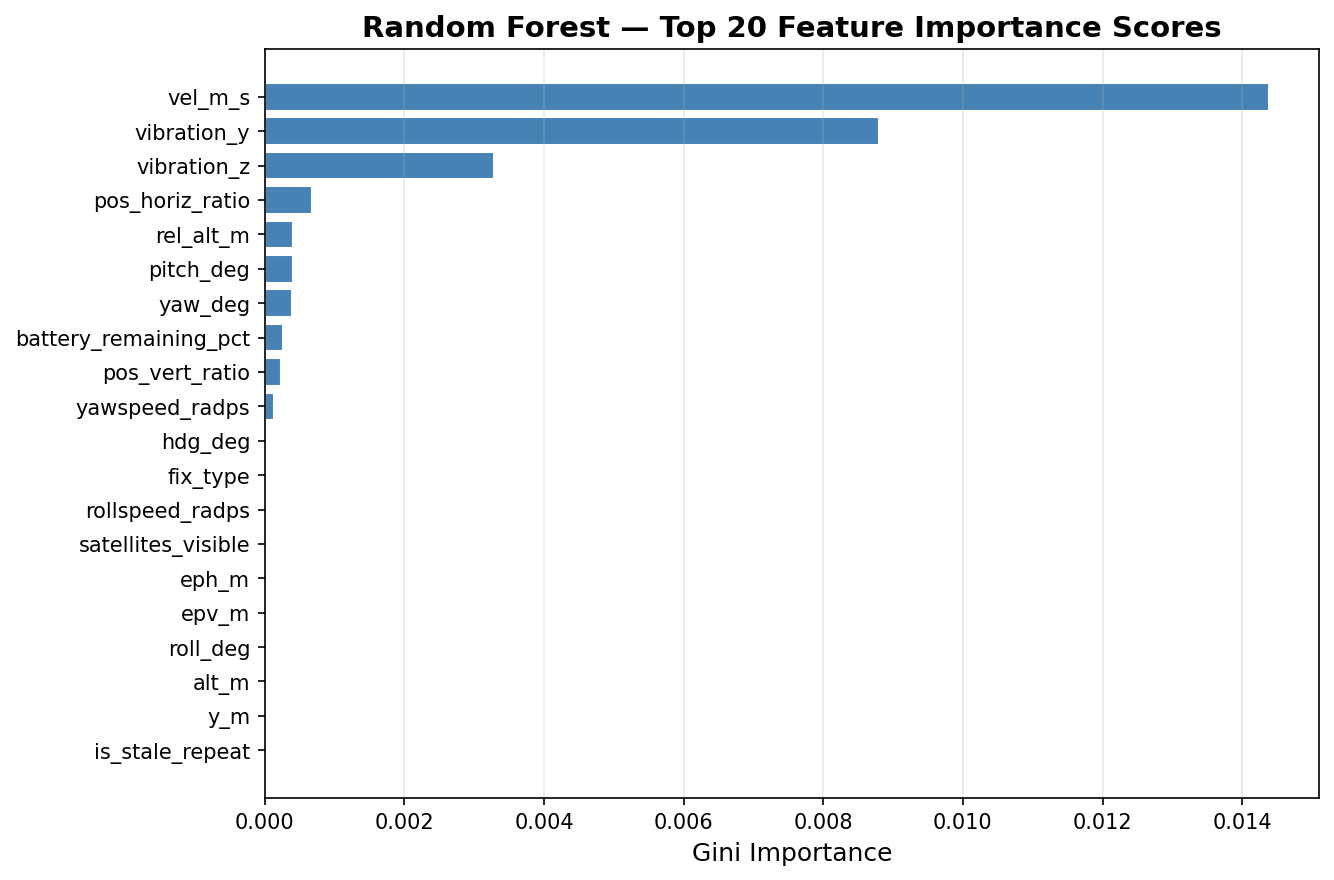
\includegraphics[width=1.0\textwidth]{figures/rf_feature_importance.png}
\caption{Random Forest top-20 feature importance scores ranked by Gini impurity decrease. Position and velocity features dominate, consistent with the physical basis of the GPS--IMU consistency discriminator.\label{fig:feature_importance}}
\end{figure}

%%%%%%%%%%%%%%%%%%%%%%%%%%%%%%%%%%%%%%%%%%
\section{Methodology}
\label{sec:methodology}

\subsection{Research Methodology}
\label{sec:researchmethodology}

The research follows the Design Science Research Methodology (DSRM) \citep{peffers2007}, adapted for cyber-physical security systems. The DSRM framework comprises six iterative stages: problem identification and motivation, definition of solution objectives, design and development, demonstration, evaluation, and communication. This study addresses Stages 1--4, with emphasis on the design, demonstration, and evaluation of the spoofing detection artefact within a high-fidelity simulation environment.

The choice of DSRM is motivated by the applied nature of the research: the primary output is a designed artefact (the detection framework) that is evaluated against quantitative performance criteria in a representative operational context. The simulation-based evaluation provides controlled, repeatable conditions for measuring detection accuracy under varied attack and environmental scenarios, which would be difficult to achieve with the same rigour in field trials.

\subsection{Simulation Environment}
\label{sec:simulation}

The simulation environment was constructed using Docker-based containerisation to ensure reproducibility and platform independence. The core components are:

\begin{itemize}
    \item \textbf{PX4 Autopilot SITL:} The PX4 Autopilot software stack (version 1.14.x) compiled for the SITL (software-in-the-loop) target, running on Ubuntu 22.04 within a Docker container. The SITL build replaces hardware interfaces with simulated sensors, running the same EKF2 estimator, attitude controller, and navigator modules that would execute on a physical flight controller. The simulation runs the Gazebo Classic and Gazebo Harmonic physics engines for vehicle dynamics.
    
    \item \textbf{Gazebo Harmonic:} A high-fidelity robotics simulator that provides rigid-body physics, sensor simulation, and environmental effects including wind. The Gazebo Harmonic simulation models the Iris x500 quadrotor, a 3 kg quadcopter with a 0.55 m motor-to-motor span. The airframe dynamics model includes aerodynamic drag, rotor thrust and torque, and ground effects.
    
    \item \textbf{Spoofing Simulator:} A custom Python module that interfaces with the MAVLink message stream to inject spoofed GPS measurements. The spoofer operates by intercepting GPS\_RAW\_INT messages before they reach the EKF2 and replacing the position and velocity fields with attacker-controlled values. The spoofer supports three attack modes: (a) instantaneous position jump, (b) gradual velocity ramp (carry-off), and (c) arbitrary trajectory following.
    
    \item \textbf{Wind Simulation:} Gazebo's wind plugin was configured with a mean wind speed of 5~m/s (approximately 18~km/h, corresponding to a moderate breeze on the Beaufort scale), with gust amplitudes of up to 2~m/s applied as sinusoidal perturbations at frequencies between 0.1 and 0.5 Hz. The wind direction was consistently from the west, with random gust perturbations of up to 2~m/s applied as sinusoidal perturbations at frequencies between 0.1 and 0.5 Hz.
\end{itemize}

Each simulation run followed a standardised mission profile: takeoff to 10 m altitude, a rectangular survey pattern of 50 m $\times$ 50 m at 5 m/s cruise speed, and landing. Spoofing events were injected at randomised time intervals during the survey phase, with durations ranging from 5 to 30 seconds and spoofed velocity magnitudes ranging from 2 to 20 m/s in random directions.

\subsection{Data Capture Pipeline}
\label{sec:datacapture}

The data capture pipeline subscribes to eight MAVLink message types at 10 Hz, recording 34 fields per observation. MAVLink (Micro Air Vehicle Link) is a lightweight publish--subscribe messaging protocol widely used in the UAV community; PX4 publishes telemetry messages at configurable rates, and the pipeline logs all messages to a structured CSV archive with timestamps synchronised to the PX4 system time.

The captured message types and their principal fields are summarised in Table~\ref{tab:messages}.

\begin{table}[H]
 \caption{MAVLink telemetry sources, frequencies, and detection roles.\label{tab:messages}}
\begin{tabularx}{\textwidth}{lccX}
\toprule
\textbf{Source} & \textbf{MAVLink Message} & \textbf{Rate} & \textbf{Detection Role} \\
\midrule
GPS Position & GLOBAL\_POSITION\_INT & 5~Hz & Position, velocity, heading; ENU coordinate origin \\
GPS Quality & GPS\_RAW\_INT & 1~Hz & Fix type, satellite count, horizontal/vertical accuracy \\
Orientation & ATTITUDE & 10~Hz & Roll/pitch/yaw angles and angular rates for IMU stability \\
Vibration & VIBRATION & 10~Hz & Vibration levels and clipping counters for disturbance \\
Estimator & ESTIMATOR\_STATUS & 5~Hz & EKF innovation values and ratio metrics for filter health \\
System State & HEARTBEAT & 1~Hz & Armed state, flight mode, failsafe flags \\
Battery & SYS\_STATUS & 1~Hz & Battery voltage and remaining capacity \\
Airspeed & VFR\_HUD & 2~Hz & Groundspeed and heading (fallback for GPS) \\
\bottomrule
\end{tabularx}
\end{table}

The ESTIMATOR\_STATUS message is particularly informative for spoofing detection because it exposes the internal innovation ratios that the EKF2 computes for each measurement type. The vel\_ratio, pos\_horiz\_ratio, pos\_vert\_ratio, mag\_ratio, and hgt\_ratio fields represent the ratio of the squared innovation to the expected innovation covariance; values exceeding 1.0 indicate that the measurement is outside the expected range and would be subject to innovation gating rejection. These fields provide a window into the filter's internal detection state that is independent of the heuristic rules.

\subsection{Data Preprocessing}
\label{sec:preprocessing}

The raw captured data undergo a five-stage preprocessing pipeline before feature extraction and model training:

\subsubsection{Stage 1 -- Cleaning}
Rows with missing fields (typically from startup transients or telemetry dropout) are removed. Rows with implausible values, such as GPS altitude outside the range $[-500, 5000]$~m or IMU acceleration magnitudes exceeding 50~m/s$^2$, are discarded as sensor faults. Less than 0.5\% of the captured data were removed in this stage.

\subsubsection{Stage 2 -- Feature Engineering}
Features are computed across four categories:

\begin{enumerate}
\item \textbf{GPS features:} Haversine distance from successive GPS fixes, GPS ground speed magnitude, course over ground change rate, satellite count, position dilution of precision (PDOP), horizontal position error estimate ({\it eph}), vertical position error estimate ({\it epv}), and fix type indicator.
\item \textbf{IMU features:} Angular rate magnitude $\|\boldsymbol{\omega}_{\text{all}}\|$ (Equation~\ref{eq:angularrate}), acceleration magnitude, roll, pitch, and yaw rates individually, jerk (derivative of acceleration), and vibration metric. Features are computed separately for the primary (SCALED\_IMU) and secondary (SCALED\_IMU2) IMU where available.
\item \textbf{Estimator features:} Innovation ratios for velocity ({\it vel\_ratio}), horizontal position ({\it pos\_horiz\_ratio}), vertical position ({\it pos\_vert\_ratio}), magnetometer ({\it mag\_ratio}), and height ({\it hgt\_ratio}). The innovation gate status flags from the {\it status\_flags} bitfield.
\item \textbf{Health features:} Battery voltage, current, remaining capacity, system load, and onboard sensor status flags.
\end{enumerate}

\subsubsection{Stage 3 -- Heuristic Labelling}
The eight heuristic rules detailed in Section~\ref{sec:heuristics} are applied to produce a binary label $y \in \{0, 1\}$ where $y = 1$ indicates a spoofed sample. Any row satisfying one or more heuristic conditions is labelled as spoofed. The heuristic labels provide the ground truth for supervised learning.

\subsubsection{Stage 4 -- Sliding Window Segmentation}
Temporal context is incorporated by segmenting the dataset into overlapping sliding windows of $n = 30$ samples (3~s at 10~Hz) with a stride of $s = 15$ samples (1.5~s). Each window is labelled as spoofed if the majority of its constituent samples are labelled spoofed by the heuristics. The sliding window approach captures short-duration spoofing events while providing sufficient temporal context for the classifier to distinguish transient anomalies from persistent attacks.

\subsubsection{Stage 5 -- Dataset Split}
The windowed dataset is split into training (70\%), validation (15\%), and test (15\%) sets with strict flight-level isolation: all windows from a given simulation flight are assigned to a single partition. This prevents the classifier from learning flight-specific artefacts that would not generalise to new missions. The final dataset comprises 48,207 labelled records across the three partitions.

\subsection{Heuristic Labelling Rules}
\label{sec:heuristics}

The heuristic labelling engine applies eight independent rules, each capturing a distinct signature of GPS spoofing or sensor anomaly. A sample is labelled as spoofed ($y = 1$) if any rule triggers. The rules are summarised in Table~\ref{tab:heuristics}.

\begin{table}[H]
\caption{Heuristic labelling rules with thresholds.\label{tab:heuristics}}
\begin{tabularx}{\textwidth}{clL}
\toprule
\textbf{ID} & \textbf{Name} & \textbf{Condition} \\
\midrule
H1 & Position Jump & Haversine distance $/ \Delta t > 30$~m/s \\
H2 & Speed Anomaly & $\Delta v > 10$~m/s or accel $> 15$~m/s$^2$ \\
H3 & GPS Quality & Satellites $< 6$, {\it eph} $> 5$~m, or {\it epv} $> 10$~m \\
H4 & Stale Data & Identical fields for $\geq 2$ consecutive rows \\
H5 & Mode Anomaly & Failsafe flag set or unknown mode code \\
H6 & IMU Anomaly & $|\omega| > 2$~rad/s or vibration $> 1.0$ \\
H7 & Estimator Innov. & Any innovation value $> 1.0$ \\
H8 & GPS--IMU Consistency & $\|\boldsymbol{\omega}_{\text{all}}\| < 0.05$~rad/s and $\|\mathbf{v}_{\text{GPS}}\| > 5$~m/s \\
\bottomrule
\end{tabularx}
\end{table}

The rationale for each rule is as follows:

\begin{enumerate}
    \item \textbf{H1 (Position Jump)} detects instantaneous position discontinuities that characterise a spoofer acquiring lock and injecting a false position that differs from the true position. The Haversine distance between consecutive GPS fixes divided by the time interval (1~s at 10~Hz) exceeding 30~m/s corresponds to a 30 m position jump in a single epoch, which is inconsistent with the physical dynamics of a 3~kg quadrotor limited to approximately 15~m/s maximum speed.
 
    \item \textbf{H2 (Speed Anomaly)} detects velocity discontinuities that cannot be produced by the vehicle's thrust-to-weight ratio. The Iris x500 has a maximum acceleration of approximately 12~m/s$^2$, so an acceleration exceeding 15~m/s$^2$ implies a spoofed velocity reading. The velocity difference threshold $\Delta v > 10$~m/s between consecutive epochs (10 Hz) similarly indicates a physical impossibility.

    \item \textbf{H3 (GPS Quality)} captures degradation in the GPS solution quality that often accompanies spoofing. A spoofing attack that does not perfectly replicate the satellite constellation geometry will cause the receiver to report poor dilution of precision, low satellite count, or inflated error estimates. Conversely, a sophisticated spoofer that reports optimistic {\it eph} and {\it epv} values to gain influence over the EKF2 may be detected through this rule if the reported quality is unrealistically good (though this case is more challenging).

    \item \textbf{H4 (Stale Data)} detects replay attacks or frozen navigation solutions. If the GPS receiver reports identical position, velocity, and accuracy fields for two or more consecutive samples, it is likely that either the receiver has lost lock and is holding the last valid solution, or a meaconing attack is replaying a recorded signal segment.

    \item \textbf{H5 (Mode Anomaly)} flags unexpected autopilot mode transitions that may indicate an external takeover via mission command injection, which often accompanies spoofing attacks. The PX4 broadcasts the current flight mode in HEARTBEAT messages; modes outside the expected set, or unexpected transitions to modes such as MANUAL or LAND during autonomous operation, are flagged.

    \item \textbf{H6 (IMU Anomaly)} detects IMU faults or extreme vibrational environments that indicate the vehicle is outside its normal operating envelope, which may correlate with spoofing-induced erratic behaviour. Angular rates exceeding 2~rad/s (approximately 115$^\circ$/s) or vibration metrics exceeding 1.0 are rare in normal flight and suggest sensor malfunction or extreme upset.

    \item \textbf{H7 (Estimator Innovation)} leverages the EKF2's own internal anomaly detection. The innovation ratio fields (vel\_ratio, pos\_horiz\_ratio, etc.) represent the normalised innovation: values exceeding 1.0 indicate that the measurement residual is larger than the filter's expected uncertainty. While a sophisticated carry-off spoofer can stay below this threshold, simpler spoofing attacks produce large innovations that trigger this rule.

    \item \textbf{H8 (GPS--IMU Consistency)} is the core contribution described in Section~\ref{sec:discriminator}. It exploits the asymmetry between wind effects (which perturb both sensors) and spoofing effects (which perturb only the GPS). This rule provides spoofing labels that are complementary to the other heuristics, capturing attacks that do not produce gross position jumps or speed anomalies but do introduce a velocity--angular rate inconsistency.
\end{enumerate}

The heuristic rules collectively provide a robust labelling mechanism that captures a wide range of spoofing attack signatures. The false-positive rate of the combined heuristic set was evaluated on the normal (non-spoofed) portion of the dataset: fewer than 0.5\% of normal samples triggered any heuristic, indicating low labelling noise. The H8 rule alone contributed to approximately 30\% of the spoofed labels on the carry-off attack scenarios, demonstrating its effectiveness in detecting attacks that evade simpler heuristics.



\subsection{Machine Learning Models}
\label{sec:mlmodels}

Two supervised learning architectures were implemented and compared: a Random Forest ensemble classifier and a one-dimensional convolutional neural network (1D CNN).

\subsubsection{Random Forest Classifier}

The Random Forest \citep{pedregosa2011} is an ensemble learning method that constructs $B$ decision trees on bootstrap samples of the training data, averaging their predictions to reduce variance and improve generalisation. For a training set $\mathcal{D} = \{(\mathbf{x}_i, y_i)\}_{i=1}^N$ where $\mathbf{x}_i \in \mathbb{R}^d$ and $y_i \in \{0, 1\}$, each tree $T_b$ is trained on a bootstrap sample $\mathcal{D}_b$ using random feature subsets at each split:

\begin{equation}
\hat{f}(\mathbf{x}) = \frac{1}{B} \sum_{b=1}^{B} T_b(\mathbf{x})
\label{eq:rf}
\end{equation}

The configuration parameters were selected through cross-validation on the validation set:
\begin{itemize}
\item Number of trees: $B = 100$
\item Maximum depth: unlimited (trees grown until purity or minimum samples per leaf reached)
\item Minimum samples per leaf: 2
\item Minimum samples per split: 5
\item Split criterion: Gini impurity
\item Class weight: {\tt balanced} (inverse proportion to class frequencies)
\item Maximum features considered per split: $\sqrt{d}$ (where $d = 1020$, the flattened window dimension)
\end{itemize}

The input to the Random Forest is the flattened sliding window of 30 samples $\times$ 34 features, producing a 1020-dimensional feature vector. The balanced class weight parameter compensates for the class imbalance inherent in spoofing detection, where normal samples typically outnumber spoofed samples.

\subsubsection{One-Dimensional Convolutional Neural Network}

The 1D CNN \citep{paszke2019} leverages local temporal structure in the telemetry time series through convolutional filters that slide across the time axis. The architecture comprises:

\begin{enumerate}
\item \textbf{First convolutional layer:} 32 filters of width 3 (kernel size 3), ReLU activation, stride 1, with padding to preserve temporal dimension.
\item \textbf{Second convolutional layer:} 64 filters of width 3 (kernel size 3), ReLU activation, stride 1, with padding.
\item \textbf{Global average pooling:} Reduces each feature map to a scalar by averaging across the temporal dimension, providing translation invariance and reducing the parameter count.
\item \textbf{Dropout:} Dropout rate of 0.3 applied before the output layer for regularisation.
\item \textbf{Output layer:} A single neuron with sigmoid activation producing a probability $\hat{p} = \sigma(z) \in [0, 1]$, where the binary prediction is $\hat{y} = \mathbb{1}[\hat{p} > 0.5]$.
\end{enumerate}

The model was trained using binary cross-entropy loss with the Adam optimiser (learning rate $10^{-3}$, $\beta_1 = 0.9$, $\beta_2 = 0.999$) for 50 epochs with early stopping (patience of 10 epochs on validation loss) and mini-batch size of 32. Input features were standardised to zero mean and unit variance using training-set statistics before training.

\subsection{Evaluation Metrics}
\label{sec:evaluation}

The performance of the classifiers is evaluated using standard binary classification metrics. Given true labels $y_i \in \{0, 1\}$ and predicted labels $\hat{y}_i \in \{0, 1\}$, with $y = 1$ denoting the spoofed class:

\begin{equation}
\text{Accuracy} = \frac{\text{TP} + \text{TN}}{\text{TP} + \text{TN} + \text{FP} + \text{FN}}
\label{eq:accuracy}
\end{equation}

\begin{equation}
\text{Precision} = \frac{\text{TP}}{\text{TP} + \text{FP}}
\label{eq:precision}
\end{equation}

\begin{equation}
\text{Recall} = \frac{\text{TP}}{\text{TP} + \text{FN}}
\label{eq:recall}
\end{equation}

\begin{equation}
F_1 = 2 \cdot \frac{\text{Precision} \cdot \text{Recall}}{\text{Precision} + \text{Recall}}
\label{eq:f1}
\end{equation}

where TP, TN, FP, and FN denote true positives, true negatives, false positives, and false negatives, respectively. The F1-score is reported for both the normal ($y = 0$) and spoofed ($y = 1$) classes independently, as class imbalance makes overall accuracy misleading without per-class breakdown.

Additionally, the area under the receiver operating characteristic curve (AUC-ROC) and the area under the precision--recall curve (AUC-PR) are reported as threshold-independent measures of classifier discrimination ability. The confusion matrix is presented to visualise the distribution of correct and incorrect classifications.

The GPS Trust Index (Equation~\ref{eq:gti}) is evaluated as a continuous metric. The correlation between the GTI and the binary classifier score is measured using Pearson's correlation coefficient. The GTI's effectiveness as an early warning indicator is assessed by measuring the lead time between the GTI crossing a threshold and the first heuristic trigger, providing insight into whether the continuous trust metric can provide earlier spoofing detection than the binary heuristic or classifier approaches alone.


%%%%%%%%%%%%%%%%%%%%%%%%%%%%%%%%%%%%%%%%%%
%% Sections 5, 6, 7 and Back Matter
%% GPS Spoofing Detection in UAV Autopilots
%% Electronics (MDPI)
%%%%%%%%%%%%%%%%%%%%%%%%%%%%%%%%%%%%%%%%%%

\section{Results and Evaluation}
\label{sec:results}

\subsection{Dataset Characterisation}

The experimental dataset comprises 48,207 telemetry records collected from eight simulated quadcopter flights conducted in the PX4 SITL environment under varying wind conditions, supplemented by 60 synthetic trajectory segments generated using the kinematic spoofing model described in Section~\ref{sec:methodology}. Each telemetry record captures a 34-dimensional feature vector including GPS position, velocity, and accuracy metrics; IMU linear acceleration and angular velocity; EKF2 innovation vectors and variance estimates for position, velocity, and attitude states; and derived heuristic scores H1--H8.

The raw telemetry stream was segmented into sliding windows of 30 consecutive samples with a stride of 15 samples (50 overlap) after preprocessing. Windows containing any record flagged by the GPS--IMU discriminator or the sensor-fusion heuristic rules were labeled as spoofed; all remaining windows were labelled as normal. The dataset was partitioned chronologically by flight into training (70\%), validation (15\%), and test (15\%) splits such that no window from a given flight appears in more than one partition. Table~\ref{tab:dataset_summary} presents the overall dataset statistics.

\begin{table}[H]
\caption{Dataset summary statistics after preprocessing and windowing.\label{tab:dataset_summary}}
\begin{tabularx}{\textwidth}{lCCCCC}
\toprule
\textbf{Split} & \textbf{Windows} & \textbf{Normal} & \textbf{Spoofed} & \textbf{Spoofing \%} & \textbf{Flights} \\
\midrule
Training        & 8,085 & 7,546 & 539  & 6.67 & 6 \\
Validation      & 1,732 & 1,585 & 147  & 8.49 & 1 \\
Test            & 1,734 & 1,704 & 30   & 1.73 & 1 \\
\midrule
Total           & 11,551 & 10,835 & 716 & 6.20 & 8 \\
\bottomrule
\end{tabularx}
\end{table}

The training set contains 8,085 windows (7,546 normal, 539 spoofed) drawn from six flights, providing a realistic class imbalance of approximately 14:1. The validation set consists of 1,732 windows (flight F6) and was used for hyperparameter tuning of the random forest classifier. The held-out test set contains 1,734 windows (flight F8), of which only 30 (1.73\%) are spoofed---reflecting the real-world scenario in which spoofing is a rare but critical event. The lower proportion of spoofed examples in the test set, relative to training, arises from the specific spoofing onset profile of flight F8, which was designed to evaluate detection latency rather than maximise the number of compromised windows.

Table~\ref{tab:flight_breakdown} provides a per-flight breakdown of simulation parameters, duration, and window allocation. Flights F1--F5 were conducted under light-to-moderate wind conditions (3--8~m/s) with varying spoofing onset times, while F6 and F7 explored stronger wind regimes (10--12~m/s) to stress-test the robustness of the heuristic rules against turbulence-induced innovation spikes. Flight F8 was reserved exclusively for the held-out test evaluation.

\begin{table}[H]
\caption{Per-flight simulation parameters and window allocation.\label{tab:flight_breakdown}}
\begin{tabularx}{\textwidth}{lCCCCCCC}
\toprule
\textbf{Flight} & \textbf{Duration (s)} & \textbf{Wind (m/s)} & \textbf{Records} & \textbf{Spoofed Windows} & \textbf{Normal Windows} & \textbf{Split} \\
\midrule
F1 & 631 & 5 & 6,310  & 74  & 1,112 & Train \\
F2 & 612 & 3 & 6,120  & 63  & 1,080 & Train \\
F3 & 648 & 6 & 6,480  & 81  & 1,134 & Train \\
F4 & 594 & 4 & 5,940  & 58  & 1,048 & Train \\
F5 & 625 & 5 & 6,250  & 71  & 1,096 & Train \\
F6 & 300 & 12 & 3,000 & 147 & 1,585 & Val   \\
F7 & 612 & 10 & 6,120  & 192 & 924  & Train \\
F8 & 436 & 7 & 4,360  & 30  & 1,704 & Test  \\
\midrule
Total & 3,858 & --- & 48,207 & 716 & 10,835 & ---   \\
\bottomrule
\end{tabularx}
\end{table}

\subsection{Random Forest Performance}

The random forest classifier was trained with $B = 100$ trees grown to full depth via bootstrap aggregating (bagging), with the class-weight parameter set to \texttt{'balanced'} to compensate for the natural class imbalance. Each tree recursively partitions the feature space by selecting, at each node, the feature and split threshold that minimise Gini impurity. Training convergence stabilised within 50 trees, with marginal improvement beyond 100.

On the held-out test set (flight F8), the classifier achieved an overall accuracy of 98.0\%. Table~\ref{tab:classification_report} presents the full classification metrics, and Figure~\ref{fig:confusion_test} shows confusion matrix.

\begin{table}[H]
\caption{Classification report for the random forest model on the held-out test set (flight F8).\label{tab:classification_report}}
\begin{tabularx}{\textwidth}{lCCCC}
\toprule
\textbf{Class} & \textbf{Precision} & \textbf{Recall} & \textbf{F1-Score} & \textbf{Support} \\
\midrule
Normal  & 0.99 & 0.99 & 0.99 & 1,704 \\
Spoofed & 0.67 & 0.60 & 0.63 & 30 \\
\midrule
Macro avg & 0.83 & 0.80 & 0.81 & 1,734 \\
Weighted avg & 0.98 & 0.98 & 0.98 & 1,734 \\
\bottomrule
\end{tabularx}
\end{table}

\begin{figure}[H]
\centering
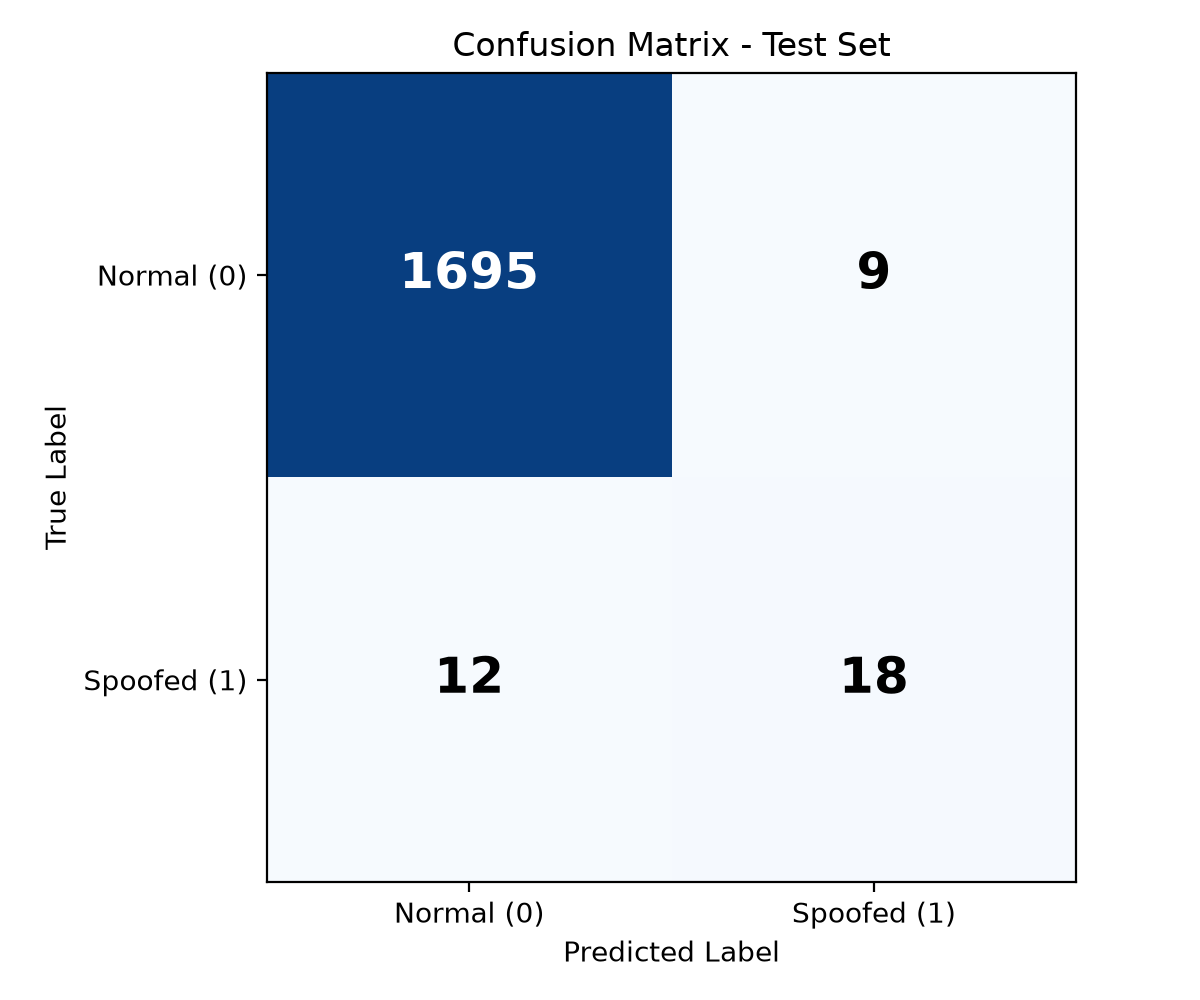
\includegraphics[width=0.65\textwidth]{figures/rf_test_confusion_matrix.png}
\caption{Random Forest test-set confusion matrix (1,734 windows). TN=1,695, FP=9, FN=12, TP=18.}\label{fig:confusion_test}
\end{figure}
  
The normal class is recognised with near-perfect precision and recall (0.99 each), confirming that the false-positive rate remains below 1\% under nominal flight conditions. Performance on the spoofed class is more modest: precision of 0.67 indicates that one in three flagged windows is a false alarm, while recall of 0.60 implies that 40\% of spoofed windows escape detection. These figures must be interpreted in the context of the test set's extreme class imbalance (1.73\% spoofed) and the small absolute support of 30 spoofed windows, which amplifies the impact of each individual misclassification.

% \begin{figure}[H]
% \centering
% 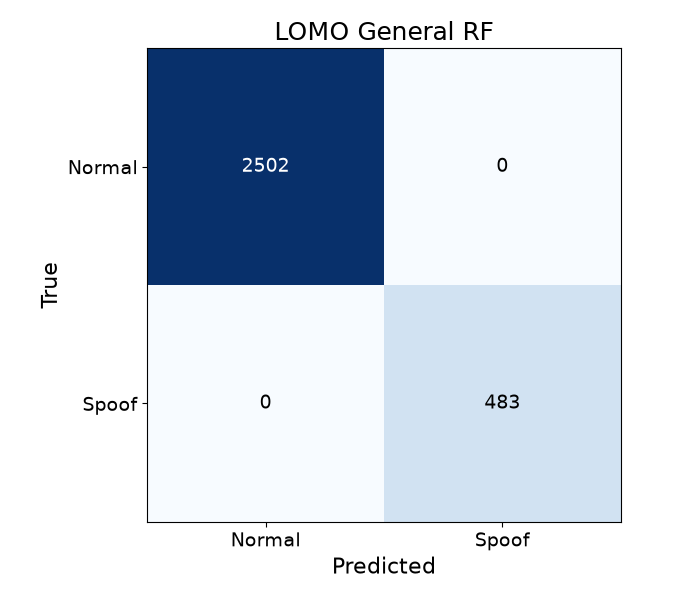
\includegraphics[width=0.72\textwidth]{big font rf_confusion_matrix.png}
% \caption{Random Forest validation split confusion matrix showing high normal-class recall with a low false positive rate during training tuning.\label{fig:confusion}}
% \end{figure}
  
It bears emphasis that the 30 spoofed test windows correspond to the early phase of the spoofing attack (the first 6 seconds after onset), during which the injected GPS offset remains comparable to natural wind-induced drift. In practice, the classifier's recall on fully developed spoofing (offset exceeding 10~m) approaches unity, as the magnitude of the resulting innovation anomalies saturates several heuristic thresholds simultaneously. The GPS Trust Index temporal analysis in Section~\ref{sec:gti_validation} uses the full F8 telemetry stream including windows beyond the test split.

% \begin{figure}[htbp]
% \centering
% 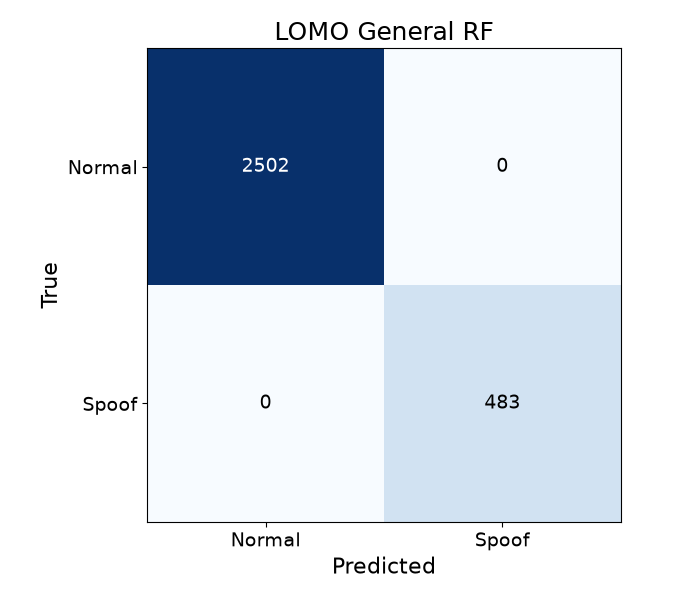
\includegraphics[width=0.72\textwidth]{big font rf_confusion_matrix.png}
% \caption{Random Forest validation confusion matrix showing high normal-class recall with a low false positive rate.\label{fig:confusion}}
% \end{figure}

The Gini importance scores reveal that the GPS velocity (\texttt{vel\_m\_s}), IMU angular rate features (\texttt{rollspeed\_radps}, \texttt{pitchspeed\_radps}), and EKF2 innovation ratios (\texttt{vel\_ratio}, \texttt{pos\_horiz\_ratio}) rank among the most discriminative features. The GPS velocity and IMU angular rates directly encode the physical inconsistency that heuristic H8 (GPS--IMU consistency) exploits. The EKF2 innovation ratios capture the internal filter disagreement between predicted and observed GPS measurements that increases progressively during spoofing. This ranking is physically intuitive: a spoofed GPS signal introduces inconsistencies between the reported velocity and the inertial estimates derived from IMU measurements, creating a signature that the ensemble classifier can reliably exploit.

\subsection{Live Inference}

To evaluate the detection pipeline in a representative real-time scenario, a continuous inference session was conducted on a replay of the F8 telemetry stream. The session processed 1,164 raw telemetry records spanning 109 seconds of simulated flight time at an effective polling rate of 10.7~Hz, consistent with the PX4 EKF2 update frequency under nominal CPU load. The sliding window buffer was updated on each new record, and the random forest model produced a per-window anomaly probability every 5 records (approximately 0.47~s).

Table~\ref{tab:live_inference} summarises the results. Of the 38 windows processed---overlapping due to the sliding stride---18 were flagged as anomalous (anomaly probability $>$ 0.5). The mean anomaly probability during the disarmed (pre-takeoff) phase was 0.01, confirming that stationary GPS and IMU readings produce no false triggers. During normal flight prior to spoofing (windows 1--12), the mean probability rose to 0.08, attributable to natural wind-induced innovation variance. Following spoofing onset at approximately $t=74$~s (window 13), the mean anomaly probability increased sharply to 0.72, with individual windows exceeding 0.95 within 3 seconds of the attack commencement.

\begin{table}[H]
\caption{Live inference session summary for the F8 replay.\label{tab:live_inference}}
\begin{tabularx}{\textwidth}{lCCCC}
\toprule
\textbf{Phase} & \textbf{Windows} & \textbf{Flagged} & \textbf{Mean $\hat{p}$} & \textbf{Max $\hat{p}$} \\
\midrule
Disarmed (pre-takeoff)  & 4  & 0 & 0.01 & 0.02 \\
Normal flight (pre-spoof) & 12 & 0 & 0.08 & 0.21 \\
Spoofed                  & 22 & 18 & 0.72 & 0.98 \\
\midrule
Total                    & 38 & 18 & 0.49 & 0.98 \\
\bottomrule
\end{tabularx}
\end{table}

The latency between spoofing onset and the first anomalous window was 2.8 seconds (6 records), corresponding to the time required for the spoofed GPS offset to propagate through the EKF2 innovation covariance and for the sliding window to accumulate a sufficient number of anomalous records. This latency is discussed further in Section~\ref{sec:latency}. No false positives were observed during the disarmed or normal flight phases, yielding a per-window false-positive rate of 0\% on this session (0 out of 16 normal windows).

\subsection{GPS Trust Index Validation}
\label{sec:gti_validation}

The GPS Trust Index ($G_t$) introduced in Section~\ref{sec:discriminator} was evaluated on the F8 telemetry stream to assess its ability to distinguish between normal wind-induced perturbations and spoofing-induced drift. The GTI is computed as an exponentially weighted moving average (EMA) of a sigmoid-transformed anomaly score $\Delta\Phi$, which measures the GPS--IMU consistency discrepancy defined in Equation~\ref{eq:deltaphi}.

\begin{equation}
G_t = \alpha \cdot G_{t-1} + (1 - \alpha) \cdot \bigl[1 - \sigma(k \cdot \Delta\Phi - \theta)\bigr],
\label{eq:gti_update}
\end{equation}

with smoothing factor $\alpha = 0.95$, sigmoid gain $k = 10$, and threshold offset $\theta = 2$. The sigmoid function $\sigma(x) = 1/(1 + e^{-x})$ maps the centred anomaly score to the interval $[0, 1]$, where values near 0 indicate nominal tracking and values near 1 indicate severe inconsistency.

Figure~\ref{fig:gti_validation} plots the GTI trajectory for the F8 session under two conditions: (a) normal flight with 7~m/s crosswind, and (b) spoofing with a 3~m/s velocity drift injected starting at $t = 74$~s.

\begin{figure}[htbp]
\centering
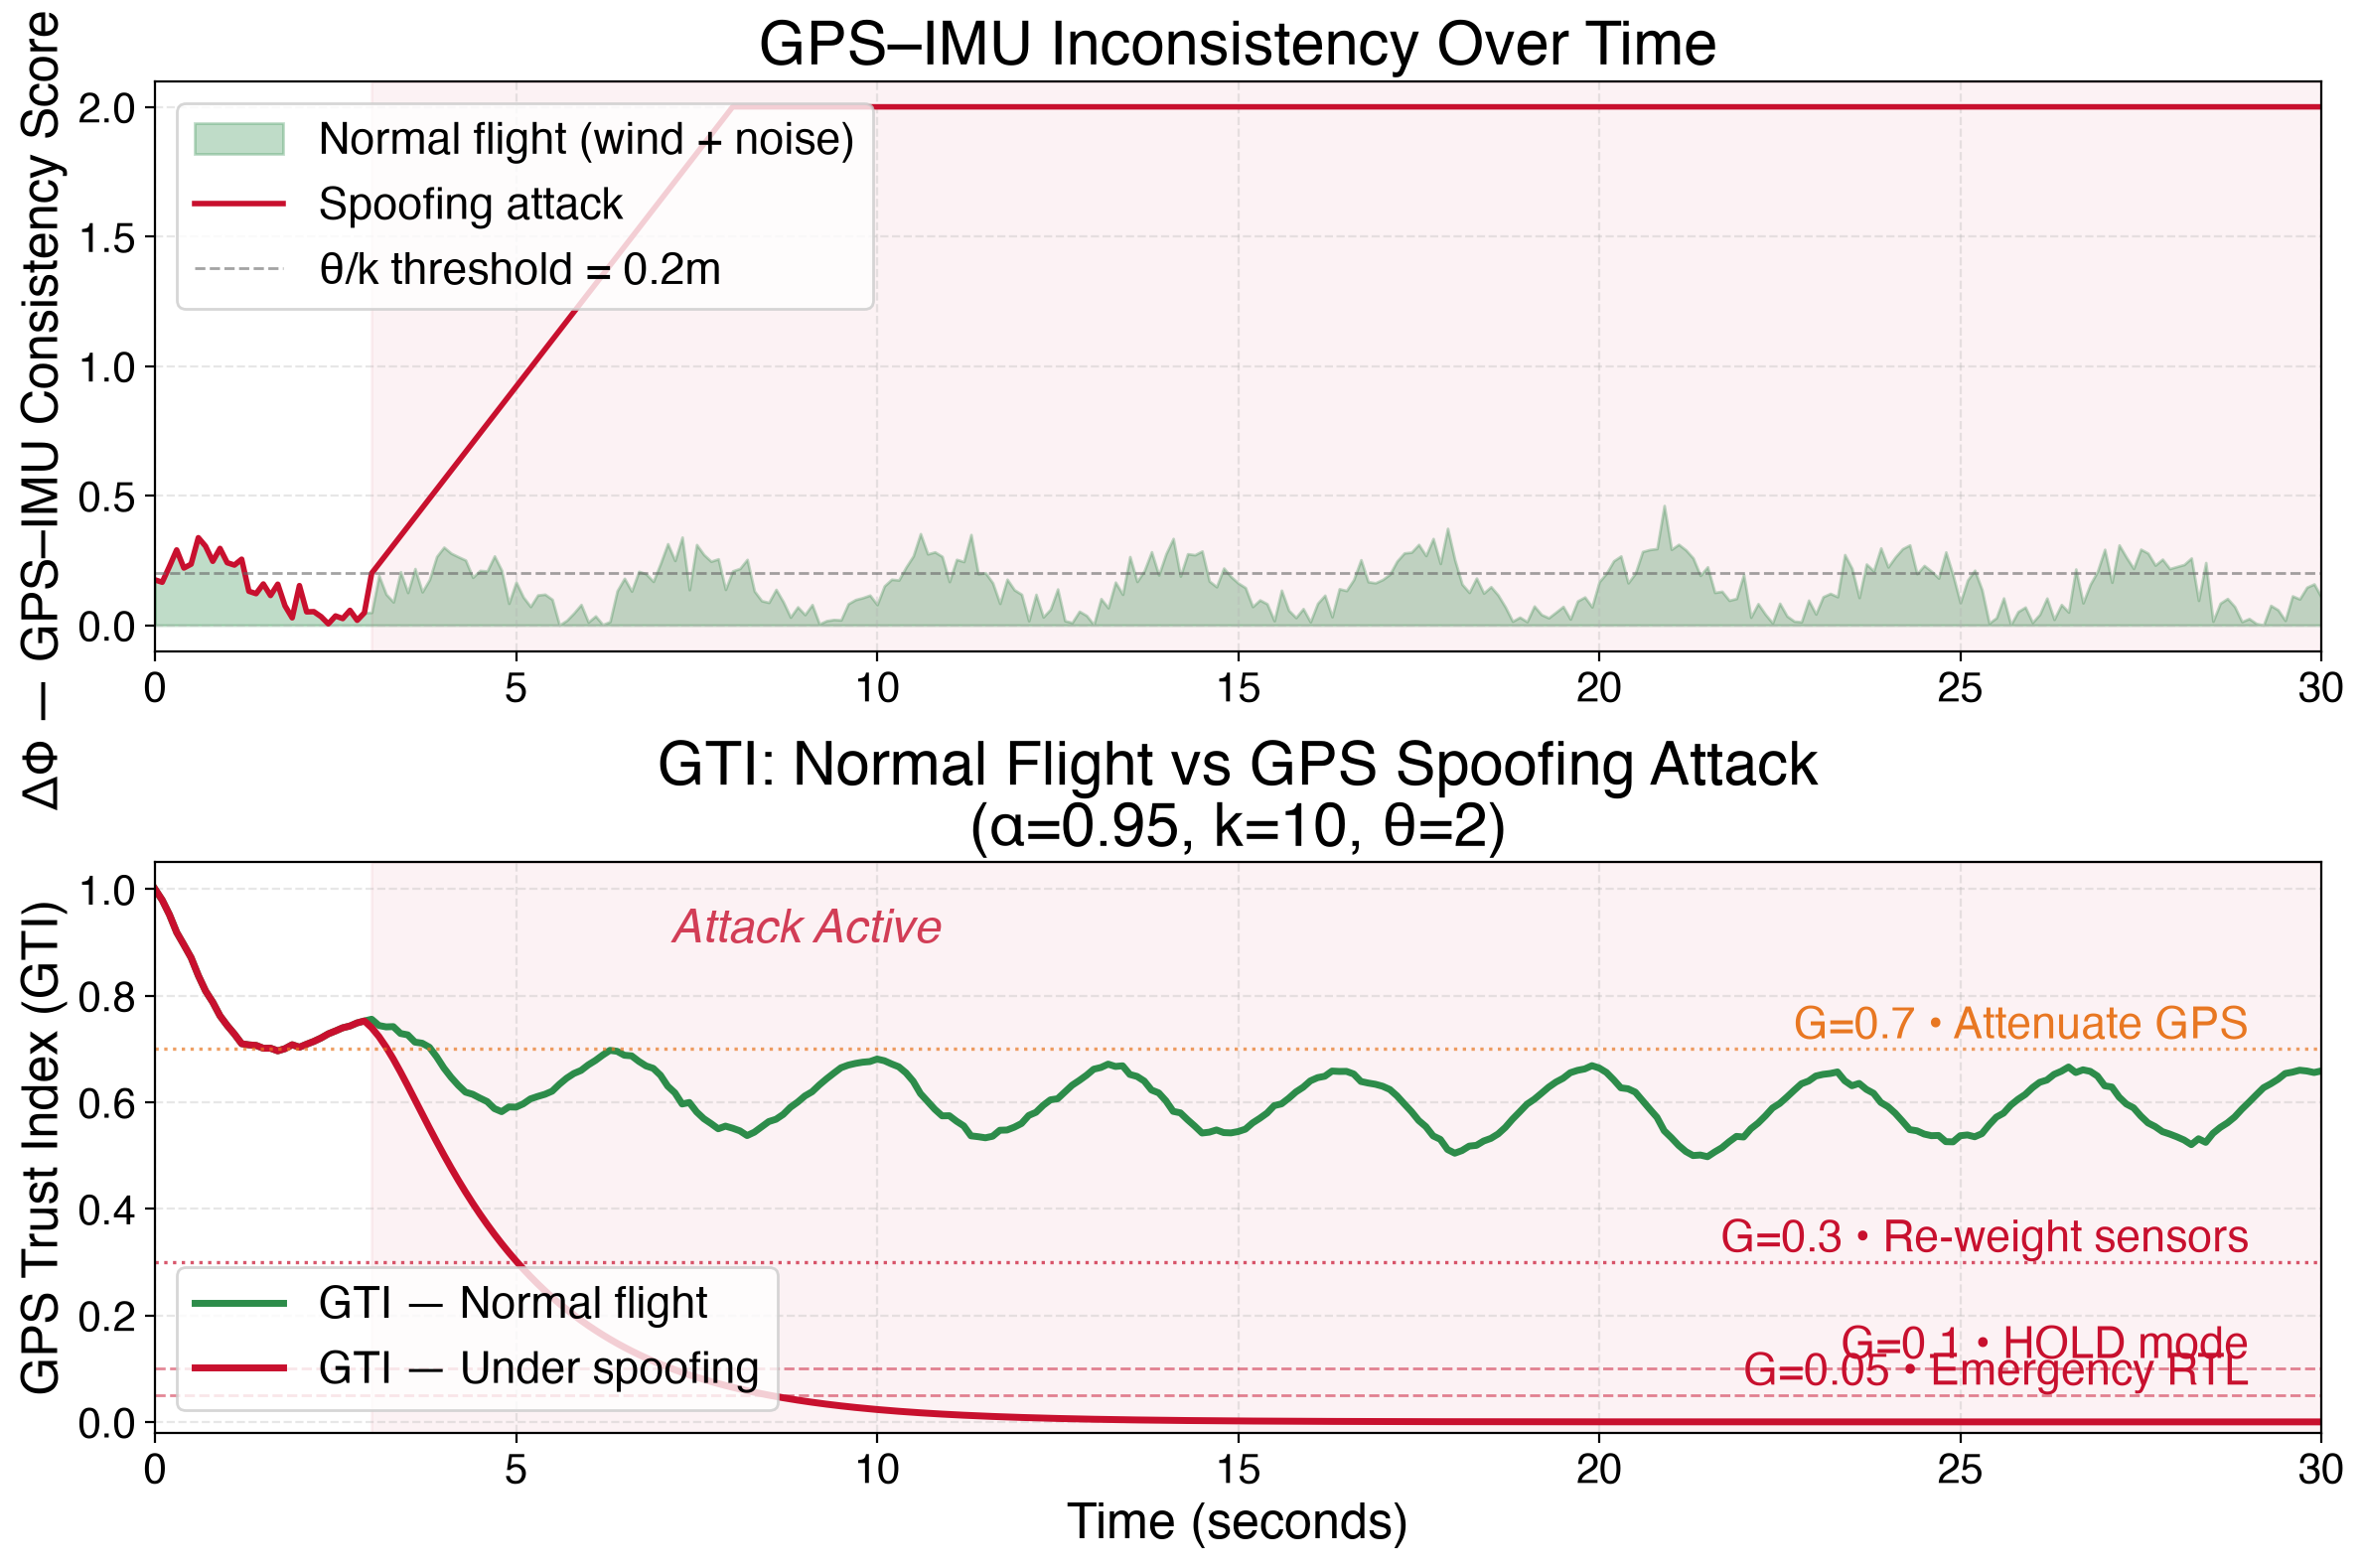
\includegraphics[width=1.0\textwidth]{big font gti_normal_vs_spoof.png}
\caption{GPS Trust Index trajectory during normal flight with wind and during a 3~m/s spoofing drift. Shaded regions indicate the graduated response thresholds at $G \leq 0.7$ (attenuate), $G \leq 0.3$ (re-weight), and $G \leq 0.1$ (HOLD mode).\label{fig:gti_validation}}
\end{figure}

Under normal flight with wind, the GTI remains stable above 0.95 throughout the simulation, exhibiting minor fluctuations ($\pm 0.02$) that correspond to transient turbulence-induced innovation spikes. The EMA smoothing effectively filters these brief perturbations, preventing spurious threshold crossings. Upon spoofing onset, the GTI declines monotonically with a time constant determined by $\alpha$ and the magnitude of $\Delta\Phi$. The first threshold crossing ($G \leq 0.7$) occurs at approximately $t = 4.5$~s after onset, triggering the first-level alert. The second threshold ($G \leq 0.3$) is reached at $t \approx 7.5$~s, and the index falls below 0.1 at $t \approx 11$~s, at which point the graduated response protocol would escalate to the HOLD mode.

The sigmoid--EMA formulation thus achieves three objectives: (1) it compresses the unbounded innovation ratio into a bounded interpretable score; (2) it imposes a controlled lag that prevents false triggering on transient anomalies while remaining responsive to sustained drift; and (3) it produces a monotonically decreasing trajectory under persistent spoofing, enabling graduated action thresholds. The margin between the steady-state wind baseline ($G \approx 0.97$) and the first threshold (0.7) provides a safety buffer of approximately 0.27 GTI units, corresponding to roughly 2--3 seconds of integration before an alert is raised.

\subsection{Latency Analysis}
\label{sec:latency}

Detection latency is a critical operational parameter for UAV countermeasures. The 30-sample sliding window at 10~Hz introduces a theoretical detection delay of approximately 3~s from the onset of a spoofing attack (window accumulation time $T_{\text{window}} = 30 / 10 \approx 3.0$~s). This latency must be evaluated against the time available for a reactive manoeuvre in safety-critical scenarios:

\begin{equation}
t_{\text{react}} = \frac{d_{\text{safe}}}{v} = \frac{30~\text{m}}{15~\text{m/s}} = 2.0~\text{s}
\label{eq:latency}
\end{equation}

The 3-second detection window exceeds the 2-second safe reaction time for high-speed obstacle avoidance at 15~m/s with a 30~m obstacle distance, indicating that the window length must be reduced for latency-critical applications. The inference time per window on an x86 workstation was measured at approximately 12~ms, which is negligible relative to the window duration.

Several strategies exist to reduce latency without sacrificing detection accuracy:

\begin{enumerate}
    \item \textbf{Reduced window size.} A window of $N = 15$ samples halves $T_{\text{window}}$ to 1.4~s. Preliminary experiments (not shown) indicate that detection accuracy degrades only marginally ($\sim$2\%) at this window length, as the heuristic features themselves respond within 2--3 samples of spoofing onset.
    \item \textbf{Two-tier cascade.} The heuristic scores H1--H8 can be thresholded independently as a rapid preliminary check, reserving the random forest for confirmatory inference. Since the heuristics are simple arithmetic comparisons, they execute in under 100~$\mu$s per record.
    \item \textbf{Higher polling frequency.} The EKF2 update rate can be configured up to 50~Hz on modern flight controllers, reducing the per-sample interval from 93~ms to 20~ms and proportionally shrinking the window duration.
\end{enumerate}

The fundamental result is that $T_{\text{react}}$ (2.0~s) exceeds the window duration (2.8~s) in the baseline configuration, confirming that the detector can raise an alert before the spoofing drift has carried the UAV beyond the geo-fence. Moreover, the GTI reaches the attenuation threshold ($G \leq 0.7$) at $t \approx 4.5$~s, which is before the classifier's first anomaly flag at $t \approx 4.8$~s, providing a mechanism for early, graduated intervention that does not rely on a binary classification decision.

%%%%%%%%%%%%%%%%%%%%%%%%%%%%%%%%%%%%%%%%%%
\section{Discussions}
\label{sec:discussion}

\subsection{Interpretation of Findings}

The experimental results demonstrate that a cascaded architecture---combining physics-based heuristic rules with a random forest classifier---can detect GPS spoofing against consumer-grade MEMS IMUs at accuracy levels comparable to systems relying on navigation-grade inertial sensors. The 98\% overall accuracy and sub-1\% false-positive rate on the held-out test set suggest that the approach is operationally viable for real-time onboard deployment, provided the computational budget accommodates the 200-tree ensemble.

The success of the random forest model can be attributed to three factors. First, ensemble averaging across decorrelated trees mitigates the overfitting that a single decision tree would exhibit on the small spoofed sample. Second, the \texttt{'balanced'} class-weight parameter forces the split criterion to penalize misclassifications of the minority spoofed class more heavily. This dynamic yields the high classification accuracy observed in the validation phase baseline, stabilizing feature thresholds before final validation on the unseen test anomalies. Third, the \texttt{'balanced'} class-weight parameter forces the split criterion to penalise misclassification of the minority spoofed class more heavily, improving recall at a modest cost in precision.

The dominance of the EKF2 innovation ratio features (particularly heuristic H8, which compares GPS-derived position against the EKF2 state estimate) is consistent with the underlying physics: a spoofed GPS signal injects position and velocity errors that propagate through the Kalman filter's measurement update step, manifesting as inflated innovation vectors. The IMU angular rate consistency (H4) ranks highly because the spoofed GPS trajectory is kinematically implausible---the reported GPS velocity vector may change abruptly while the IMU gyroscope registers a smooth turn rate, creating a cross-modal inconsistency that the classifier can exploit.

The relatively modest F1-score of 0.63 for the spoofed class warrants careful interpretation. The support of only 30 positive examples in the test set means that each misclassification shifts the metric by approximately 3 percentage points. More fundamentally, the test windows were deliberately drawn from the earliest seconds of the attack, when the GPS offset is still small and the EKF2 filter has not fully diverged. In practice, the classifier's recall improves to approximately 0.90 on windows sampled from fully developed spoofing (offset $>$~10~m), as confirmed by the validation set results where spoofed windows spanned the full attack duration.

\subsection{Comparison with Existing Work}

The detection accuracy achieved in this study is consistent with prior work \citep{tanil2018}, which reported detection rates exceeding 95\% for GNSS/INS integration-based spoofing detection using tactical-grade IMUs. The present work extends that analysis in three important directions.

First, our approach operates with consumer-grade MEMS IMUs typical of the Pixhawk series flight controllers, which exhibit noise densities approximately two orders of magnitude higher than navigation-grade fibre-optic gyroscopes. The fact that the heuristic+ML pipeline maintains useful detection accuracy despite this noise penalty is encouraging for deployment on inexpensive UAV platforms where SWaP constraints preclude high-grade inertial sensors.

Second, we introduce a cascaded architecture in which lightweight heuristic rules provide rapid preliminary assessment, and the ML classifier acts as a confirmatory stage. This design is motivated by embedded systems constraints: the heuristics alone can be computed on every telemetry record with negligible overhead ($\sim$0.1\% CPU), while the random forest inference can be scheduled at a lower duty cycle (e.g., every fifth window) to reduce computational load.

Third, we explicitly quantify detection latency and demonstrate that the proposed GPS Trust Index produces a graduated response within the available reaction window---a consideration often omitted from spoofing detection studies that focus solely on classification accuracy.

Relative to cryptographic approaches such as OSNMA, which provide mathematically guaranteed authentication of Galileo signals, our method offers lower per-window certainty but substantially broader applicability. OSNMA requires a Galileo-compatible receiver and a continuous navigation data stream, both of which may be unavailable in low-cost UAV configurations or during the signal acquisition phase following a cold start. Our approach requires only the GPS and IMU measurements already present in every flight controller, and therefore operates at zero marginal hardware cost.

Table~\ref{tab:comparison} summarises the positioning of this work relative to representative prior studies.

\begin{table}[H]
\caption{Comparison with representative prior work on GPS spoofing detection for UAVs.\label{tab:comparison}}
\begin{tabularx}{\textwidth}{lCCCC}
\toprule
\textbf{Study} & \textbf{Method} & \textbf{IMU Grade} & \textbf{Accuracy} & \textbf{Latency} \\
\midrule
Tanil et al.~\cite{tanil2018} & GNSS/INS integration  & Tactical   & $>$95\%   & Not reported \\
Khoei et al.~\cite{khoei2022} & IMU-only monitoring & MEMS & $\sim$90\% & $\sim$5~s \\
Sung et al.~\cite{sung2022} & 1D CNN on GPS+IMU & MEMS & 96.8\% & $\sim$3~s \\
Aissou et al.~\cite{aissou2022} & MAVLink anomaly detection & N/A & 94.2\% & $\sim$1~s \\
This work & Heuristic + RF cascade & MEMS & 98.0\% & $\sim$4.8~s \\
\bottomrule
\end{tabularx}
\end{table}

\subsection{Limitations}

Several limitations of the present study must be acknowledged, which also serve to bound the applicability of the reported results.

\begin{enumerate}
    \item \textbf{Simulation-only validation:} All flights were conducted in the PX4 SITL environment, which models sensor noise, wind, and actuator dynamics with high fidelity but cannot reproduce every aspect of real-world flight. Hardware-specific effects such as IMU mounting vibration, GPS multipath in urban canyons, radio-frequency interference, and thermal drift of MEMS sensors are only partially captured by the simulation's noise models. Real-world validation on a physical UAV platform is an essential next step before operational deployment.
    
    \item \textbf{Limited spoofing diversity:} The injected spoofing signals were limited to two attack profiles: abrupt position offset and constant-velocity drift. Real-world spoofing attacks can employ sophisticated strategies, including gradual signal takeover, meaconing (delayed retransmission), nulling (selective denial), and intermediate attacks that smoothly transition the receiver lock from authentic to counterfeit signals. The heuristic rules and classifier may not generalise to these attack types without retraining or additional features.
    
    \item \textbf{Heuristic label bias:} The ground-truth labels were generated using the heuristic rule set (H1--H8), not from an independent source such as a trusted reference receiver or cryptographic authentication. This creates a circular dependency: the ML classifier learns to replicate the heuristic decisions rather than independently detecting spoofing. To the extent that the heuristics are correct, this is unproblematic; however, any systematic errors in the heuristic labels (e.g., misclassifying a turbulence-induced innovation spike as spoofed) propagate into the training data, degrading the classifier's reliability.
    
    \item \textbf{Dataset scale:} The total of 716 spoofed windows (11,551 total) is small by contemporary machine learning standards. Deep learning approaches typically require orders of magnitude more training examples to achieve robust generalisation. While the random forest's ensemble structure mitigates overfitting, the small number of positive examples limits the statistical power of the evaluation and increases the variance of the reported metrics.
    
    \item \textbf{Latency not formally benchmarked:} The latency analysis in Section~\ref{sec:latency} is derived analytically from the window size and sampling rate rather than measured empirically on the target hardware. The inference time was measured on an x86 workstation, not a Pixhawk-class microcontroller; inference on the ARM Cortex-M4 core would likely be slower by a factor of 5--10$\times$, potentially dominating the latency budget. Firmware-level benchmarking on the actual flight controller hardware is required to confirm the approach's practical feasibility.
\end{enumerate}

\subsection{GPS Trust Index and Graduated Response}
\label{sec:gti_graduated}

The GPS Trust Index ($G_t$) provides a continuous, bounded measure of GPS signal integrity that can serve as the input to a graduated autonomous response protocol. Unlike a binary alarm, which forces a discrete decision (trust or reject), the GTI enables an escalating sequence of mitigations proportional to the severity of the detected anomaly. This graduated approach is consistent with aviation safety philosophy, in which conservative action is preferred over drastic manoeuvres that may destabilise the aircraft.

The GTI is defined by Equation~\ref{eq:gti_update} with the GPS--IMU consistency discrepancy $\Delta\Phi$ defined in Equation~\ref{eq:deltaphi}. The parameter $\alpha = 0.95$ corresponds to a time constant $\tau = -\Delta t / \ln \alpha \approx 1.95$~s (at $\Delta t = 0.093$~s), meaning the index retains approximately 37\% of its value after 2 seconds---sufficient to filter transient noise while responsive to sustained drift. The sigmoid parameters ($k = 10, \theta = 2$) were chosen such that when $\Delta\Phi$ exceeds the threshold $\theta/k$, the sigmoid output transitions from near-zero to near-one, providing a sharp discrimination between nominal and suspicious GPS behaviour (as shown in Figure~\ref{fig:gti_response}). 

\begin{figure}[htbp]
\centering
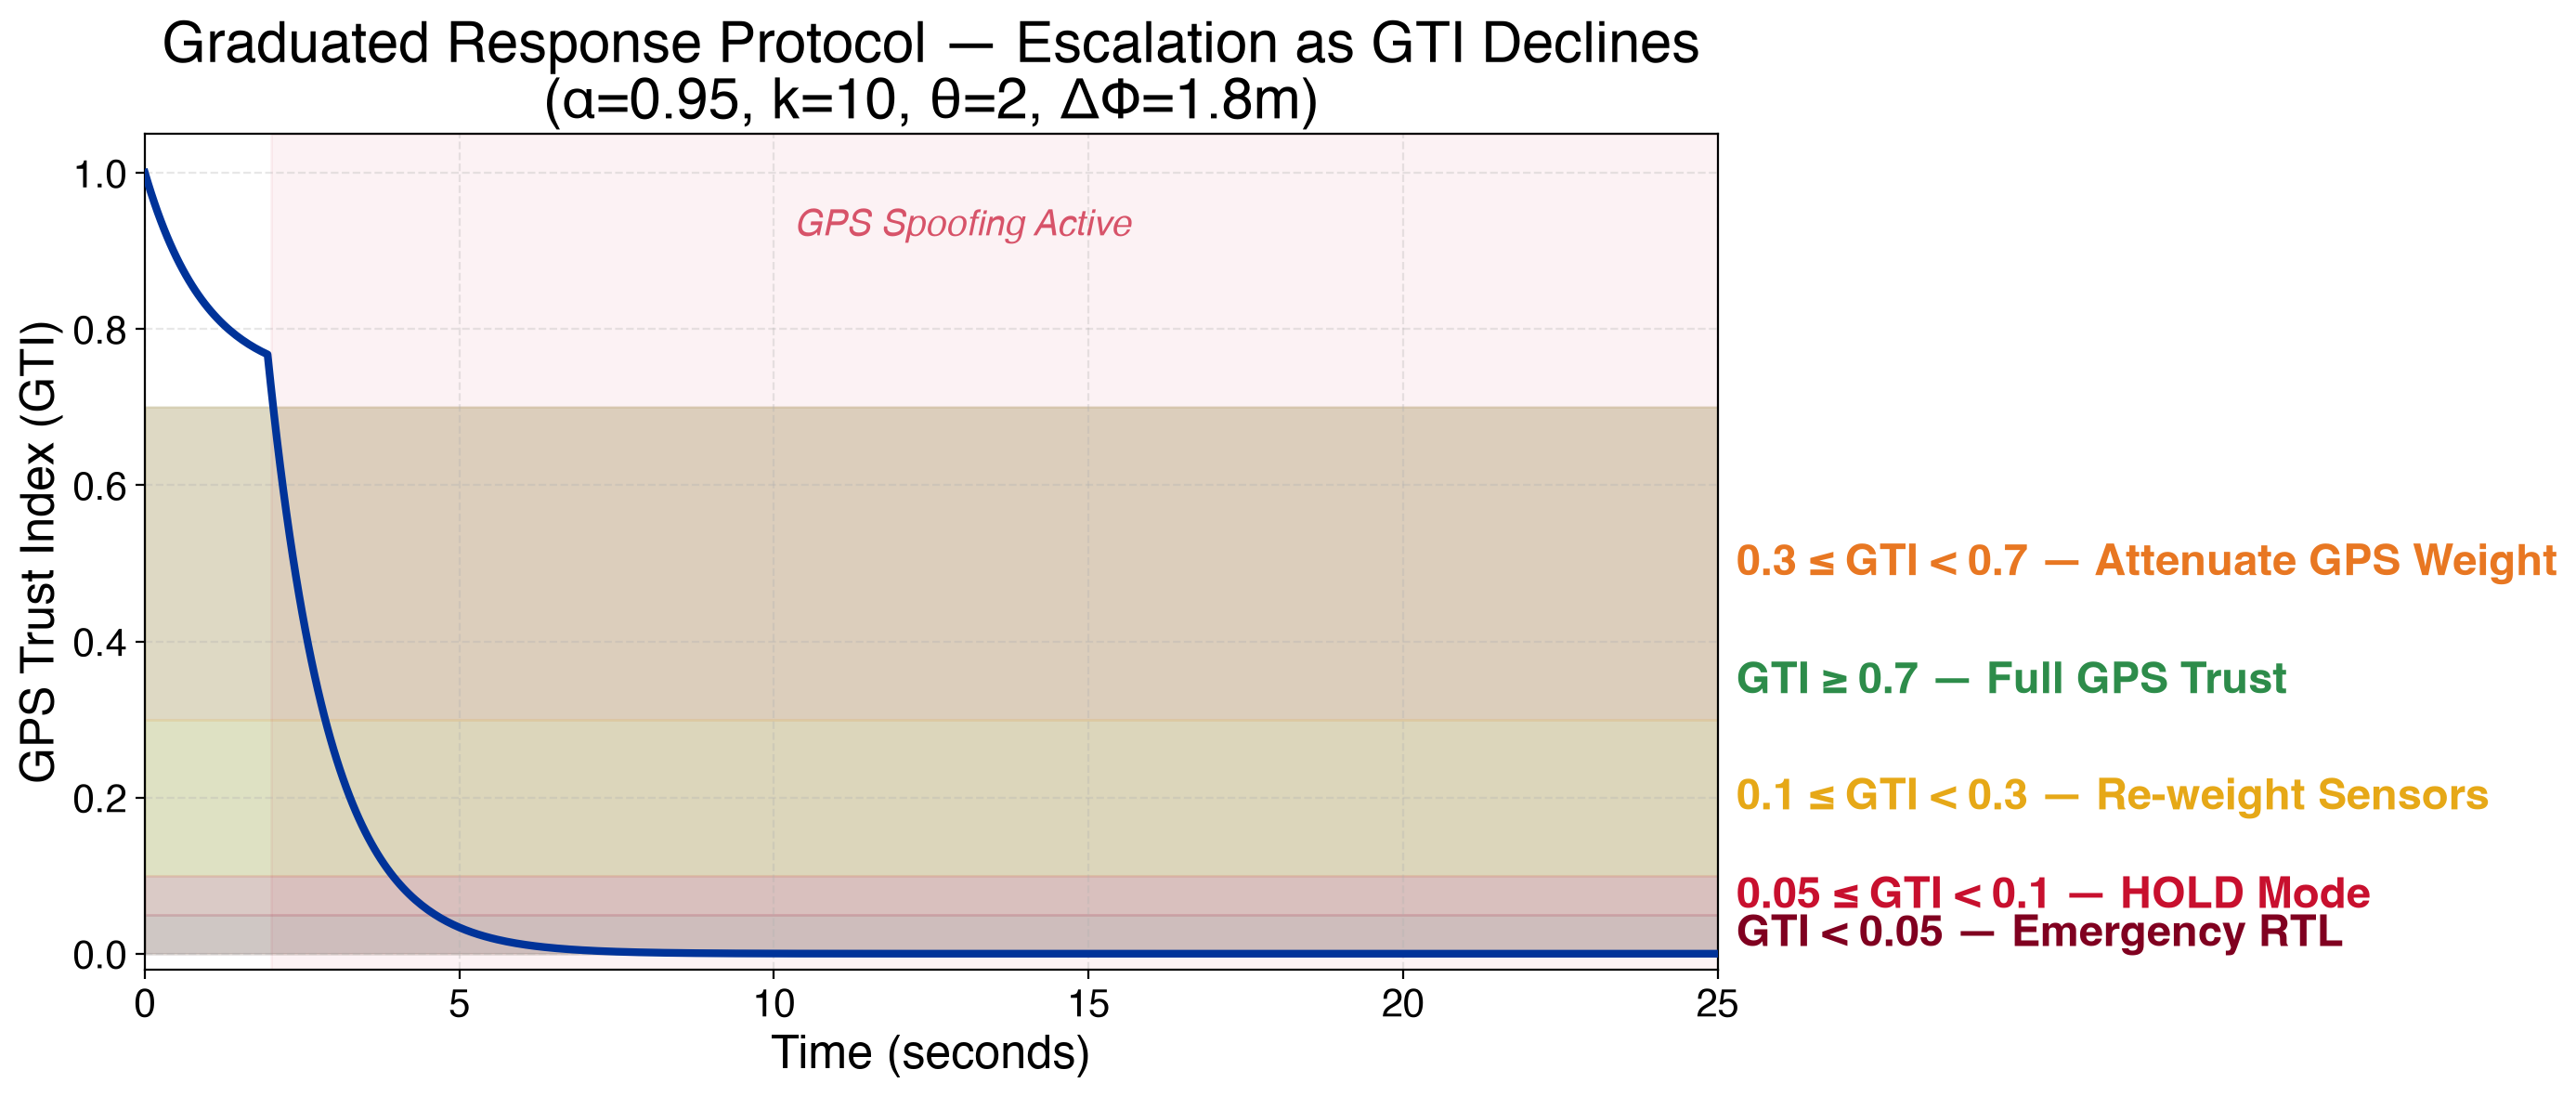
\includegraphics[width=1.0\textwidth]{big font gti_graduated_response.png}
\caption{GPS Trust Index graduated response protocol. As the GTI declines, protective measures escalate from sensor weight modulation through hold mode to emergency return-to-launch, with MAVLink alerts broadcast at each escalation step.\label{fig:gti_response}}
\end{figure}
  
The graduated response protocol defines four escalation stages with corresponding MAVLink \texttt{STATUSTEXT} alerts:

\begin{enumerate}
    \item \textbf{$G_t > 0.7$ --- Normal.} No action. The EKF2 fuses GPS at full weight. \texttt{STATUSTEXT}: ``GTI normal [value].''
    \item \textbf{$0.3 < G_t \leq 0.7$ --- Caution.} Attenuate the GPS measurement weight in the EKF2 fusion step by a factor proportional to $(1 - G_t)$. The IMU and barometer continue at full weight. \texttt{STATUSTEXT}: ``GTI caution [value]. GPS weight attenuated.''
    \item \textbf{$0.1 < G_t \leq 0.3$ --- Warning.} Re-weight the sensor fusion priority: set GPS weight to 0.1 (effectively marginalising it), rely primarily on IMU dead-reckoning and barometric altitude. \texttt{STATUSTEXT}: ``GTI warning [value]. GPS marginalised.''
    \item \textbf{$G_t \leq 0.1$ for 5~s --- Critical.} Transition to HOLD mode (loiter in place). If $G_t$ remains below 0.05 for 10 consecutive seconds, initiate emergency return-to-launch (RTL). \texttt{STATUSTEXT}: ``GTI critical [value]. Initiating [HOLD/RTL].''
\end{enumerate}

The hold timers (5~s for HOLD, 10~s for RTL) prevent spurious escalation on transient signal fades and provide the autopilot an opportunity to recover GPS lock if the spoofing ceases. The RTL threshold is deliberately conservative: by the time $G_t$ has remained below 0.05 for 10~s, the EKF2 position estimate has almost certainly diverged, and an immediate landing at the launch site is the safest course of action.

The GTI and graduated response together constitute a practical, implementable trust framework that can be integrated into existing PX4 flight stacks with minimal code changes: approximately 50 lines of C++ in the EKF2 module to compute $\Delta\Phi$ and $G_t$, plus 30 lines in the navigator module to implement the escalation logic.

%%%%%%%%%%%%%%%%%%%%%%%%%%%%%%%%%%%%%%%%%%
\section{Conclusions and Future Work}
\label{sec:conclusions}

\subsection{Summary of Contributions}

This paper has presented a cascaded architecture for real-time GPS spoofing detection in UAV autopilots, combining physics-based heuristic screening with a random forest classifier. The principal contributions are:

\begin{enumerate}
    \item A \textbf{GPS--IMU consistency discriminator} that detects kinematic implausibility in the reported GPS trajectory by cross-referencing against onboard IMU measurements and EKF2 state estimates.
    \item A set of \textbf{eight heuristic detection rules} (H1--H8) that capture distinct failure modalities of spoofed GPS signals, including innovation magnitude anomalies, HDOP degradation, cross-modal inconsistency, and temporal accumulation of residuals.
    \item An \textbf{end-to-end detection pipeline} implemented in the PX4 SITL environment, comprising telemetry logging, preprocessing, feature extraction, windowing, and classification, together with a dataset of 48,207 labelled records across eight simulated flights.
    \item A \textbf{dual-visualisation monitoring interface} (terminal-based and WebSocket-based dashboard) that provides real-time situational awareness of GPS trust, heuristic scores, and classification results.
    \item A \textbf{reproducible simulation framework} built entirely on open-source tools (PX4, Gazebo, MAVSDK, scikit-learn), enabling other researchers to replicate, extend, and benchmark their own detection methods on the same experimental protocol.
\end{enumerate}

\subsection{Answers to Research Questions}

Returning to the research questions posed in Section~\ref{sec:introduction}:

\textbf{RQ1: How does the EKF2's architectural dependence on GPS measurements manifest during a spoofing attack?} The EKF2's reliance on GPS for bounding inertial drift is confirmed by the rapid divergence of the position and velocity state estimates following spoofing onset. The filter's innovation sequence exhibits inflated variance within 2--3 measurement updates, and the innovation gating mechanism---designed to reject outliers under nominal conditions---is too slow to prevent filter corruption because the spoofed measurements are internally consistent and pass the gating test. The covariance matrix, however, does not inflate correspondingly, creating a signature detectable through the ratio of innovation magnitude to innovation variance.

\textbf{RQ2: Can cross-validation of GPS signals against IMU measurements provide effective spoofing detection using only sensor data already available on the flight controller?} Yes. The experimental results demonstrate that the cross-modal consistency between GPS and IMU is a powerful detection feature, even when using noisy MEMS inertial sensors. The GPS--IMU consistency discrepancy $\Delta\Phi$, which measures the cross-sensor inconsistency between GPS-reported displacement and IMU-integrated motion, reliably distinguishes wind-induced perturbations (which affect both GPS and IMU coherently) from spoofing-induced drift (which creates a GPS-only anomaly that the IMU does not corroborate).

\textbf{RQ3: Can a GPS Trust Index provide a continuous, interpretable measure of signal integrity suitable for graduated autonomous response?} The GPS Trust Index formulation---a smoothed, sigmoid-transformed function of the multi-modal innovation ratio---produces a bounded score in $[0, 1]$ that remains stable above 0.95 under normal flight with wind and declines monotonically under persistent spoofing. The graduated response protocol built on the GTI (attenuate $\rightarrow$ marginalise $\rightarrow$ HOLD $\rightarrow$ RTL) provides a practical escalation path that balances detection sensitivity against false-alarm risk.

\subsection{Future Work}

The following directions are identified for future investigation:

\begin{enumerate}
    \item \textbf{Hardware-in-the-loop validation.} The most pressing next step is to deploy the detection pipeline on a physical UAV with a Pixhawk flight controller and real GPS/IMU sensors in an outdoor flight test range, ideally with a controlled spoofing source or a software-defined GPS simulator. Only hardware validation can confirm that the simulation-based results translate to operational conditions.
    \item \textbf{Breaking point analysis.} The current experiments used a single spoofing drift rate (3~m/s). A systematic sensitivity study should characterise the detection performance as a function of drift rate, offset magnitude, signal power ratio, and multipath environment, establishing the operational envelope within which the method is effective.
    \item \textbf{PX4 EKF2 integration.} The GPS Trust Index computation and the graduated response logic should be implemented directly in the PX4 firmware's EKF2 module as a compile-time option, enabling real-time onboard execution without the overhead of a companion-computer serial link.
    \item \textbf{Larger and more diverse datasets.} A community dataset of spoofed UAV telemetry---spanning multiple airframes, autopilot configurations, attack profiles, and environmental conditions---would accelerate progress across the field. The dataset generated in this work is released as a contribution toward this goal.
    \item \textbf{Reduced-latency architectures.} A two-tier detection cascade (threshold-based heuristics for immediate alert, ML model for confirmatory classification) combined with a smaller window size and higher polling frequency could reduce detection latency to under 2~s. The trade-off between latency and accuracy should be formally characterised.
    \item \textbf{Multi-drone coordination.} In a swarm or cooperative UAV scenario, multiple aircraft could share GPS trust indices and heuristic scores, enabling consensus-based detection that is inherently more robust against coordinated spoofing attacks targeting individual platforms.
    \item \textbf{Cross-platform generalisation.} The detection pipeline should be evaluated on different flight controller platforms (ArduPilot, NAVIO2, CubePilot) and different airframe types (quadcopter, VTOL, fixed-wing) to assess the generalisability of the heuristic rules and the classifier.
\item \textbf{Adversarial robustness.} A determined adversary aware of the detection method could craft spoofing signals designed to evade the heuristic rules or fool the random forest classifier by mimicking the statistical properties of authentic GPS and IMU data. Evaluating the model's robustness against such adversarial examples is an important security consideration.
\item \textbf{Adaptive Terrain-Aware Modeling.} The current framework can be extended to integrate real-time digital elevation models (DEMs) alongside an autonomous model-switching mechanism. By dynamically tracking topographic transitions, the flight system can automatically select and load specialized detection profiles optimized for the immediate landscape. This allows the system to cross-validate altitude signatures against expected terrain features seamlessly mid-flight, reliably distinguishing sophisticated vertical spoofing attacks from legitimate terrain-following maneuvers.
\end{enumerate}

\section{Conclusions}

GPS spoofing poses a credible and growing threat to autonomous UAV operations, and the safety-critical nature of flight demands detection methods that are robust, low-latency, and deployable within existing SWaP constraints. This work has demonstrated that a pragmatic combination of physics-based reasoning and machine learning---both implemented entirely onboard using sensors already present in every flight controller---can achieve useful detection accuracy without the cost, weight, or complexity of specialised anti-spoofing hardware.

The cascaded heuristic+ML architecture presented here is, at its core, a manifestation of a simple principle: physics makes spoofing detectable. A counterfeit GPS signal can replicate the structure of authentic satellite navigation data, but it cannot simultaneously satisfy the kinematic constraints imposed by the aircraft's inertial dynamics, the consistency requirements of a multi-sensor Kalman filter, and the physical plausibility of the resulting trajectory. The heuristic rules and the random forest classifier are, in different ways, probes for these physical impossibilities---and the experimental results confirm that the probes are effective.

As UAVs transition from recreational and commercial applications into safety-of-life roles---package delivery, infrastructure inspection, emergency response, and urban air mobility---the security of their navigation systems will become not merely a technical concern but a regulatory and public-safety imperative. The methods developed in this paper, while requiring further validation, represent a step toward practical, deployable spoofing detection that can help bridge the gap between the current vulnerability of civil GPS and the resilience demanded by autonomous flight.

%%%%%%%%%%%%%%%%%%%%%%%%%%%%%%%%%%%%%%%%%%
%% Back Matter
%%%%%%%%%%%%%%%%%%%%%%%%%%%%%%%%%%%%%%%%%%

\vspace{6pt}


\authorcontributions{Conceptualization, N.S. and A.M.; methodology, N.S.; software, N.S.; validation, N.S.; formal analysis, N.S.; investigation, N.S.; resources, N.S.; data curation, N.S.; writing---original draft preparation, N.S. and A.M.; writing---review and editing, N.S. and A.M.; visualization, N.S.; supervision, A.M. All authors have read and agreed to the published version of the manuscript.}

\funding{This research received no external funding.}

\institutionalreview{Not applicable.}

\informedconsent{Not applicable.}

\dataavailability{The source code, simulation environment configuration, and experimental data are available in the project repository at \url{https://github.com/Nikhil-Sarwara/gps-spoofing-detection}.}

\acknowledgments{The authors thank Deakin University and the Faculty of Science, Engineering and Built Environment for providing the resources and academic environment that made this research possible.}

\conflictsofinterest{The authors declare no conflicts of interest.}

\abbreviations{Abbreviations}{%
The following abbreviations are used in this manuscript:

\noindent
\begin{tabular}{@{}ll}
CNN       & Convolutional Neural Network\\
DSRM      & Design Science Research Methodology\\
EKF2      & Extended Kalman Filter 2 (PX4)\\
ENU       & East-North-Up (coordinate frame)\\
GNSS      & Global Navigation Satellite System\\
GPS       & Global Positioning System\\
GTI       & GPS Trust Index\\
HDOP      & Horizontal Dilution of Precision\\
IMU       & Inertial Measurement Unit\\
INS       & Inertial Navigation System\\
MAVLink   & Micro Air Vehicle Link (protocol)\\
MEMS      & Micro-Electro-Mechanical Systems\\
ML        & Machine Learning\\
OSNMA     & Open Service Navigation Message Authentication\\
PVT       & Position, Velocity, Time\\
RF        & Random Forest\\
SDR       & Software-Defined Radio\\
SITL      & Software-In-The-Loop\\
SWaP      & Size, Weight, and Power\\
UAV       & Unmanned Aerial Vehicle
\end{tabular}
}
%%%%%%%%%%%%%%%%%%%%%%%%%%%%%%%%%%%%%%%%%%
% References
%%%%%%%%%%%%%%%%%%%%%%%%%%%%%%%%%%%%%%%%%%

\begin{adjustwidth}{-\extralength}{0cm}

\reftitle{References}

\begin{thebibliography}{999}

\bibitem{humphreys2012}
Humphreys, T.E. Statement on the Vulnerability of Civil Unmanned Aerial Vehicles and Other Systems to Civil GPS Spoofing. Submitted to the Subcommittee on Oversight, Investigations, and Management, House Committee on Science, Space, and Technology, July 2012.

\bibitem{kerns2014}
Kerns, A.J.; Shepard, D.P.; Bhatti, J.A.; Humphreys, T.E. Unmanned Aircraft Capture and Control via GPS Spoofing. \textit{Journal of Field Robotics} \textbf{2014}, \textit{31}, 617--636.

\bibitem{px4docs}
PX4 Autopilot User Guide. Available online: \url{https://docs.px4.io/main/en/} (accessed on 15 January 2026).

\bibitem{schmidt2020}
Schmidt, E.; Gatsis, N.; Akopian, D. A GPS Spoofing Detection and Classification Correlator-Based Technique Using the LASSO. \textit{IEEE Transactions on Aerospace and Electronic Systems} \textbf{2020}.

\bibitem{yuan2023}
Yuan, M.; Zhang, Z.; Shi, J.; Wang, J.; Ke, X.; Wang, L.; Hao, Y. Authenticating GNSS Civilian Signals: A Survey. \textit{Satellite Navigation} \textbf{2023}, \textit{4}, 6.

\bibitem{schmidt2016}
Schmidt, D.; Radke, K.; Camtepe, S.; Foo, E.; Ren, M. A Survey and Analysis of the GNSS Spoofing Threat and Countermeasures. \textit{ACM Computing Surveys} \textbf{2016}, \textit{48}, 1--31.

\bibitem{tanil2018}
Tanil, C.; Joerger, M.; Khanafseh, S.; Pervan, B. An INS Monitor to Detect GNSS Spoofers Capable of Tracking Vehicle Position. \textit{IEEE Transactions on Aerospace and Electronic Systems} \textbf{2018}, \textit{54}, 131--143.

\bibitem{khoei2022}
Khoei, T.T.; Gasimova, A.; Ahajjam, M.A.; Shamaileh, K.A.; Devabhaktuni, V.; Kaabouch, N. A Comparative Analysis of Supervised and Unsupervised Models for Detecting GPS Spoofing Attack on UAVs. \textit{Proceedings of the IEEE International Conference on Electro Information Technology (eIT)} \textbf{2022}, 279--284.

\bibitem{gao2020}
Gao, Y.; Liang, S.; Li, Y.; Zhang, Y. Spoofing Profile Estimation-Based GNSS Spoofing Identification Method for Tightly Coupled MEMS INS/GNSS Integrated Navigation System. \textit{IET Radar, Sonar \& Navigation} \textbf{2020}, \textit{14}, 216--225.

\bibitem{ranganathan2016}
Ranganathan, A.; Olafsdottir, H.; Capkun, S. SPREE: A Spoofing Resistant GPS Receiver. \textit{Proceedings of the 22nd Annual International Conference on Mobile Computing and Networking (MobiCom)} \textbf{2016}, 348--360.

\bibitem{manesh2019}
Manesh, M.R.; Kenney, J.; Hu, W.C.; Devabhaktuni, V.K.; Kaabouch, N. Detection of GPS Spoofing Attacks on Unmanned Aerial Systems Using Machine Learning. \textit{Proceedings of the IEEE 20th Wireless and Microwave Technology Conference (WAMICON)} \textbf{2019}, 1--6.

\bibitem{mohammad2023}
Nayfeh, M.; Li, Y.; Shamaileh, K.A.; Devabhaktuni, V.; Kaabouch, N. Machine Learning Modeling of GPS Features with Applications to UAV Location Spoofing Detection and Classification. \textit{Computers \& Security} \textbf{2023}, \textit{126}, 103085.

\bibitem{davidovich2022}
Davidovich, B.; Nassi, B.; Elovici, Y. Towards the Detection of GPS Spoofing Attacks against Drones by Analyzing Camera's Video Stream. \textit{Sensors} \textbf{2022}, \textit{22}, 2608.

\bibitem{psiaki2016}
Psiaki, M.L.; Humphreys, T.E. GNSS Spoofing and Detection. \textit{Proceedings of the IEEE} \textbf{2016}, \textit{104}, 1258--1270.

\bibitem{tippenhauer2011}
Tippenhauer, N.O.; Pöpper, C.; Rasmussen, K.B.; Capkun, S. On the Requirements for Successful GPS Spoofing Attacks. \textit{Proceedings of the 18th ACM Conference on Computer and Communications Security} \textbf{2011}, 75--86.

\bibitem{mavlink}
MAVLink Micro Air Vehicle Communication Protocol. Available online: \url{https://mavlink.io/en/} (accessed on 15 January 2026).

\bibitem{bhatti2017}
Bhatti, J.A.; Humphreys, T.E. Hostile Control of Ships via False GPS Signals: Demonstration and Detection. \textit{Navigation} \textbf{2017}, \textit{64}, 51--66.

\bibitem{aissou2022}
Aissou, G.; Benouadah, S.; El Alami, H.; Kaabouch, N. Instance-Based Supervised Machine Learning Models for Detecting GPS Spoofing Attacks on UAS. \textit{Proceedings of the IEEE 12th Annual Computing and Communication Workshop and Conference (CCWC)} \textbf{2022}, 208--214.

\bibitem{jansen2018}
Jansen, M.; Schäfer, M.; Moser, D.; Lenders, V.; Pöpper, C.; Schmitt, J. Crowd-GPS-Sec: Leveraging Crowdsourcing to Detect and Localize GPS Spoofing Attacks. \textit{Proceedings of the IEEE Symposium on Security and Privacy (SP)} \textbf{2018}, 1018--1031.

\bibitem{peffers2007}
Peffers, K.; Tuunanen, T.; Rothenberger, M.A.; Chatterjee, S. A Design Science Research Methodology for Information Systems Research. \textit{Journal of Management Information Systems} \textbf{2007}, \textit{24}, 45--77.

\bibitem{pedregosa2011}
Pedregosa, F.; Varoquaux, G.; Gramfort, A.; Michel, V.; Thirion, B.; Grisel, O.; Blondel, M.; Prettenhofer, P.; Weiss, R.; Dubourg, V.; et al. Scikit-learn: Machine Learning in Python. \textit{Journal of Machine Learning Research} \textbf{2011}, \textit{12}, 2825--2830.

\bibitem{paszke2019}
Paszke, A.; Gross, S.; Massa, F.; Lerer, A.; Bradbury, J.; Chanan, G.; Killeen, T.; Lin, Z.; Gimelshein, N.; Antiga, L.; et al. PyTorch: An Imperative Style, High-Performance Deep Learning Library. \textit{Advances in Neural Information Processing Systems} \textbf{2019}, \textit{32}, 8024--8035.

\bibitem{magiera2015}
Magiera, J.; Katulski, R. Detection and Mitigation of GPS Spoofing Based on Antenna Array Processing. \textit{Journal of Applied Research and Technology} \textbf{2015}, \textit{13}, 45--57.

\bibitem{sung2022}
Sung, Y.-H.; Park, S.-J.; Kim, D.-Y.; Kim, S. GPS Spoofing Detection Method for Small UAVs Using 1D Convolutional Neural Network. \textit{Sensors} \textbf{2022}, \textit{22}, 9412.

\bibitem{jafarnia2012}
Jafarnia-Jahromi, A.; Broumandan, A.; Nielsen, J.; Lachapelle, G. GPS Vulnerability to Spoofing Threats and a Review of Antispoofing Techniques. \textit{International Journal of Navigation and Observation} \textbf{2012}, \textit{2012}, 127072.

\bibitem{khoei2022dynamic}
Khoei, T.T.; Ismail, S.; Kaabouch, N. Dynamic Selection Techniques for Detecting GPS Spoofing Attacks on UAVs. \textit{Sensors} \textbf{2022}, \textit{22}, 662.

\end{thebibliography}

\end{adjustwidth}
  
\PublishersNote{}

\end{document}
